% =============================================================================
% Hidden Currents: A Peak-Stress Water Index for Auditing AI Data Center
% Sustainability and Informing Disclosure Policy
%
% Author: Hrihaan Bhutani
% Version 3 (preprint), October 2026. Paper: CC BY 4.0. Code: MIT.
% =============================================================================

\documentclass[conference,10pt]{IEEEtran}
\usepackage[T1]{fontenc}
\usepackage[utf8]{inputenc}
\usepackage{amsmath, amssymb, amsfonts, amsthm}
\usepackage{graphicx}
\graphicspath{{./}{../figures/}}
\usepackage{booktabs}
\usepackage{array}
\usepackage{cite}
\usepackage{url}
\usepackage{xcolor}
\usepackage{tcolorbox}
\usepackage{hyperref}

\hypersetup{colorlinks=true, linkcolor=blue!60!black,
            citecolor=blue!60!black, urlcolor=blue!60!black,
            pdftitle={Hidden Currents: A Peak-Stress Water Index for Auditing AI Data Center Sustainability},
            pdfauthor={Hrihaan Bhutani}}

\begin{document}

\title{Hidden Currents: A Peak-Stress Water Index for Auditing AI Data Center Sustainability and Informing Disclosure Policy}

\author{
\IEEEauthorblockN{Hrihaan Bhutani}
\IEEEauthorblockA{Emerald High School, Dublin, California, USA \\
hribhu19@gmail.com \\
Data and code: \url{https://github.com/hrihaan19/pswi-data-center-audit} \\
Preprint, version 3, October 2026. Not peer reviewed.}
}

\maketitle
\thispagestyle{plain}
\pagestyle{plain}

% ============================================================================
\begin{abstract}
% ============================================================================
Data center water use is usually reported as Water Usage Effectiveness (WUE),
an annual, fleet-averaged ratio of water to IT energy. WUE hides two
dimensions of impact on host communities: the concentration of demand on peak
summer days and the scarcity of water where a facility is located. Prior work
has examined these dimensions separately. We propose the \emph{Peak-Stress
Water Index} (PSWI), the product of annual WUE, a peaking factor $\beta$
(peak-day to average-day water use), and the facility's Baseline Water Stress
(BWS) from WRI Aqueduct~4.0. We apply PSWI to an open dataset of 48
hyperscale and colocation facilities run by seven operators in North America,
Europe, and Asia, using only WUE values that operators publish or that can be
derived from their published totals. Because none of these operators
publishes facility-level WUE, facilities inherit fleet or regional values, so
PSWI isolates how location changes the burden behind the same headline
number. PSWI spans a factor of about 1{,}500 across facilities; within one
operator that applies a single fleet WUE, it differs 267-fold between
Henderson, Nevada and Hamina, Finland. Company rankings by mean PSWI depart
from rankings by operator WUE (Spearman $\rho = 0.71$), although bootstrap
intervals for individual company shifts include zero. Our climate-based
$\beta$ is strongly correlated with BWS ($r = 0.84$); removing it leaves
facility and company rankings nearly unchanged ($\rho = 0.96$ for both), so
the results are driven mainly by location stress. In an idealized
reallocation exercise, moving 10\% of workload from the highest- to the
lowest-PSWI facilities lowers aggregate PSWI by 35\% (95\% interval
21--46\% under assumed input uncertainty), showing that impact is
concentrated in a small tail. None of the audited operators publishes peak or
monthly water data. We outline a facility-level disclosure framework that
borrows the phase-in architecture of U.S.\ securities disclosure rules but
could be implemented through state and local water permitting. Data and code
are openly released.
\end{abstract}

\begin{IEEEkeywords}
data centers, sustainable computing, water stress, water usage effectiveness,
AI infrastructure, environmental disclosure, sensitivity analysis
\end{IEEEkeywords}

% ============================================================================
\section{Introduction}
\label{sec:introduction}
% ============================================================================

The rapid expansion of artificial intelligence has been accompanied by a
rapid expansion of the data center infrastructure that powers it. Recent
projections place U.S.\ data center electricity consumption at 6.7\% to
12.0\% of national totals by 2028~\cite{lbnl2024}, and the International
Energy Agency projects global data center electricity demand to roughly
double by 2030~\cite{iea2025}. Water demand is growing alongside. Han et
al.\ estimate that, if 2024 water-use intensity persists, U.S.\ data centers
could require 697 to 1{,}451 million gallons per day of new public water
capacity through 2030---comparable to New York City's average daily supply of
roughly 1{,}000 million gallons---with a total valuation on the order of
\$10 billion and up to \$58 billion in a high-growth case~\cite{han2026}.

The industry's primary water metric, Water Usage Effectiveness
(WUE)~\cite{greengrid2011wue}, divides annual site water use by annual IT
energy. It is usually reported as a single fleet-wide
average~\cite{microsoft2025efficiency, meta2025edi, aws2023summary}, and it
treats every liter as equivalent. This obscures two dimensions of impact:

\begin{enumerate}
    \item \textbf{Temporal concentration of demand.} Han et
        al.~\cite{han2026} show that data center water demand is
        concentrated on the hottest days of the year, with daily peaking
        factors estimated at roughly 3 to 10 depending on climate and cooling
        configuration. Public water systems are sized for peak demand, so a
        low annual WUE can coexist with heavy peak-day draws.
    \item \textbf{Spatial heterogeneity of stress.} A liter consumed in the
        Phoenix area, in a Colorado River basin that has experienced
        persistent drought since about 2000, does not carry the same
        consequences as a liter at Hamina, Finland, where Google cools with
        seawater. Wu et al.'s SCARF framework~\cite{wu2025scarf} weights
        water consumption by a location-specific stress factor derived from
        the World Resources Institute's Aqueduct
        dataset~\cite{kuzma2023aqueduct}.
\end{enumerate}

These dimensions have been studied largely separately: Han et al.\ analyze
peak demand and system capacity without weighting by basin-level water
stress, while Wu et al.\ weight by stress without modeling peak-day
concentration. To our knowledge, no published metric combines them.

\subsection{Contributions}

\begin{enumerate}
    \item \textbf{A composite metric.} We define the \emph{Peak-Stress Water
        Index} (PSWI) as the product of annual WUE, a peaking factor, and
        Baseline Water Stress, combining the peaking framing of Han et al.\
        with the stress weighting of Wu et al.\ (Section~\ref{sec:metric}).
    \item \textbf{An auditable dataset with documented provenance.} We
        assemble 48 facilities operated by seven providers. Every WUE value
        is either published by the operator or derived arithmetically from
        published totals, and is labeled accordingly
        (Section~\ref{sec:methodology}).
    \item \textbf{Findings with explicit robustness tests.} We document a
        roughly 1{,}500-fold range in PSWI, a 267-fold difference between two
        facilities of one operator sharing a single fleet WUE, and
        departures between WUE-based and PSWI-based company rankings. We
        test these against perturbation and removal of the peaking factor,
        bootstrap resampling, and inclusion of indirect (Scope~2) water
        (Section~\ref{sec:results}).
    \item \textbf{A disclosure audit and policy framework.} None of the
        seven operators publishes peak or monthly water data. We propose
        facility-level disclosure requirements and discuss implementation in
        light of the history of the U.S.\ Securities and Exchange
        Commission's climate disclosure rules (Section~\ref{sec:policy}).
\end{enumerate}

% ============================================================================
\section{Background}
\label{sec:background}
% ============================================================================

\subsection{Data Center Water Use}

Data centers use water directly, mostly for on-site cooling, and indirectly
through electricity generation~\cite{li2023thirsty, han2026}. Evaporative
cooling removes heat efficiently by evaporating water; dry cooling avoids
on-site water use but generally requires more electricity, especially on hot
days, so the two resources trade off~\cite{karimi2022water, han2026}.
Indirect (Scope~2) water use often exceeds direct use in
volume~\cite{li2023thirsty}, but it is drawn at power plants, frequently in
other basins and largely outside public drinking-water systems. We focus on
direct use and test sensitivity to Scope~2 in Section~\ref{sec:scope2}.

\subsection{The WUE Metric and Its Limitations}

The Green Grid defines WUE as~\cite{greengrid2011wue}
\begin{equation}
\textrm{WUE} = \frac{\textrm{Annual site water usage (L)}}
                    {\textrm{Annual IT equipment energy (kWh)}}.
\label{eq:wue}
\end{equation}
As used in corporate reporting, WUE has three limitations for assessing
local impact. \textbf{Annualization} erases the peak signal that matters for
systems sized to peak demand. \textbf{Location-blindness} treats a liter in
a drought-stressed basin like a liter drawn from the Baltic.
\textbf{Aggregation} into fleet or regional averages dilutes high-impact
sites with low-impact ones. Operators also define the numerator
differently---some use water withdrawal, others consumption---which limits
comparability across companies~\cite{meta2025edi}.

% ============================================================================
\section{Related Work}
\label{sec:related}
% ============================================================================

\paragraph{Sustainable AI and computing}
Strubell et al.~\cite{strubell2019energy} documented the energy footprint of
training large language models; Patterson et al.~\cite{patterson2022carbon}
extended this to carbon. Wu et al.~\cite{wu2022sustainable} provided an
industry perspective from Meta, Schwartz et al.~\cite{schwartz2020green}
introduced the Green AI framing, and Luccioni et
al.~\cite{luccioni2023bloom} performed a life-cycle carbon analysis of
BLOOM. Most of this literature treats water as secondary to carbon or omits
it.

\paragraph{Geographical load balancing}
Islam et al.~\cite{islam2018water} exploited spatio-temporal diversity to
reduce water use in geo-distributed data centers. Acun et
al.~\cite{acun2023carbon} introduced Carbon Explorer, Radovanovi\'{c} et
al.~\cite{radovanovic2023carbon} described Google's carbon-aware computing
system, and Hanafy et al.~\cite{hanafy2024going} quantified the cost of
reducing cloud carbon emissions. Li et al.~\cite{li2024equitable} proposed
equity-aware geographical load balancing, Liu et al.~\cite{liu2024gsr}
studied geographical server relocation, and Bian et
al.~\cite{bian2024cafe} applied carbon-aware federated learning. In this
line of work, water is usually treated through unweighted volumes.

\paragraph{Water-aware computing}
Wu et al.'s SCARF framework~\cite{wu2025scarf} defines the Adjusted Water
Impact (AWI), which multiplies on-site and off-site water consumption by a
water stress factor derived from Aqueduct~\cite{kuzma2023aqueduct}. Jiang et
al.'s WaterWise~\cite{jiang2025waterwise} co-optimizes carbon and water
footprints in scheduling, and ThirstyFLOPS~\cite{jiang2025thirsty} models
the water footprint of HPC systems. Han et al.~\cite{han2026} quantify data
centers' peak demands on U.S.\ public water systems, estimate daily peaking
factors, and argue that available peak capacity rather than annual volume is
the binding constraint. Li et al.~\cite{li2023thirsty} estimate the water
footprint of AI models. De Vries-Gao~\cite{devries2026} estimates the global
water footprint of AI systems (312.5--764.6 billion liters in 2025) and
reviews which environmental metrics major operators disclose; our disclosure
audit (Section~\ref{sec:disclosure}) is narrower, asking whether the
specific inputs needed for a facility-level PSWI are published. Siddik et
al.~\cite{siddik2021environmental} estimate the environmental footprint of
U.S.\ data centers, and Karimi et al.~\cite{karimi2022water} examine
water--energy trade-offs in hot-arid climates.

\paragraph{Our contribution}
PSWI combines the peak and stress dimensions in a single facility-level
index and applies it to a cross-operator dataset whose inputs are fully
traceable to public documents.

% ============================================================================
\section{The PSWI Metric}
\label{sec:metric}
% ============================================================================

\subsection{Definition}

For facility $i$,
\begin{equation}
\textrm{PSWI}_i \;=\; \textrm{pWUE}_i \cdot \textrm{BWS}_i
\;=\; \textrm{WUE}_i \cdot \beta_i \cdot \textrm{BWS}_i ,
\label{eq:pswi}
\end{equation}
where $\textrm{WUE}_i$ is annual WUE in L/kWh; $\beta_i \geq 1$ is the daily
peaking factor, the ratio of peak-day to average-day water use; and
$\textrm{BWS}_i$ is Aqueduct~4.0's baseline water stress, the dimensionless
ratio of total water demand to available renewable
supply~\cite{kuzma2023aqueduct}. We write
$\textrm{pWUE}_i = \textrm{WUE}_i \cdot \beta_i$ for the peak-day water
intensity implied by the peaking factor; this notation is ours, building on
the peaking-factor analysis of Han et al.~\cite{han2026}. PSWI has units of
L/kWh and can be read as \emph{stress-weighted peak-day water intensity}.

\subsection{Rationale for the Multiplicative Form}

Each factor scales the previous one: $\beta$ converts average-day to
peak-day water intensity, and BWS weights each liter by the scarcity of
water where it is drawn. A product is therefore the natural composite. It
reduces to stress-weighted water intensity when $\beta = 1$, the logic of
Wu et al.'s AWI~\cite{wu2025scarf}, and to peak water intensity when BWS is
held fixed, the logic of Han et al.~\cite{han2026}. An additive index would
require arbitrary weights to combine quantities measured in different
units. The multiplicative form is a modeling choice rather than an empirical
finding; Section~\ref{sec:betasens} reports how much our results depend on
the $\beta$ component.

\subsection{Properties}

\paragraph{Monotonicity}
For positive inputs, PSWI is strictly increasing in each factor with the
others held fixed, since
$\partial\,\textrm{PSWI}/\partial X_k = \prod_{j\neq k} X_j > 0$ for
$X_k \in \{\textrm{WUE}, \beta, \textrm{BWS}\}$.

\paragraph{Log-additivity}
Because $\log\textrm{PSWI} = \log\textrm{WUE} + \log\beta + \log\textrm{BWS}$,
the cross-facility variance decomposes exactly as
\begin{equation}
\textrm{Var}(\log\textrm{PSWI}) =
\sum_k \textrm{Var}(\log X_k) + 2 \sum_{j<k} \textrm{Cov}(\log X_j, \log X_k).
\label{eq:vardecomp}
\end{equation}

\paragraph{Rank invariance under uniform rescaling}
Multiplying any factor by the same constant at every facility rescales every
PSWI equally and leaves rankings unchanged. Only differences \emph{between}
facilities in a factor can affect rankings.

\paragraph{Limiting behavior}
As $\textrm{BWS} \to 0$, $\textrm{PSWI} \to 0$ regardless of water volume,
reflecting negligible freshwater scarcity. When $\textrm{BWS} > 1$, demand
already exceeds renewable supply and PSWI exceeds pWUE.

\subsection{Known Limitations of the Metric}

\begin{tcolorbox}[colback=yellow!8, colframe=yellow!50!black,
                  title=Box 1: Known limitations in this application]
\small
\textbf{Assumed peaking factor.} $\beta$ is assigned by climate class, not
measured. It is strongly correlated with BWS across our sample ($r = 0.84$
in logs), so location enters PSWI twice. Removing $\beta$ entirely changes
facility rankings little ($\rho = 0.96$; Section~\ref{sec:betasens}). \\[2pt]
\textbf{No facility-level WUE.} No operator in our sample publishes it;
each facility inherits its operator's fleet or regional value. \\[2pt]
\textbf{Water stress inputs.} BWS values are annual, rounded, and assigned
manually by metropolitan area. \\[2pt]
\textbf{Scope 2 excluded.} Indirect water is omitted from the main
specification and tested in Section~\ref{sec:scope2}.
\end{tcolorbox}

% ============================================================================
\section{Methodology}
\label{sec:methodology}
% ============================================================================

\subsection{Sample Frame and Inclusion Criteria}

We include a facility if (i)~it is a hyperscale or major colocation data
center; (ii)~its operator publishes WUE at the fleet or regional level, or
publishes fleet totals from which WUE can be derived; (iii)~its location is
publicly known at least to the metropolitan level; (iv)~it was operating
during the reporting year; and (v)~it lies within Aqueduct~4.0 coverage. We
excluded xAI, whose Memphis facility has drawn public attention but for
which we found no published WUE, and Chinese hyperscalers, whose published
water data we could not link to facilities.

The resulting purposive sample contains 48 facilities: Google (15),
Microsoft (8), Meta (8), Amazon Web Services (6), Equinix (6), Digital
Realty (3), and QTS (2). Thirty-two are in the United States, 11 in Europe,
and 5 in Singapore and Taiwan. The sample is not statistically
representative of global capacity, and we draw no inferences about operators
that do not disclose.

\subsection{WUE Assignment}

Table~\ref{tab:wue} lists the WUE applied to each operator's facilities and
its source. No operator in the sample publishes WUE for individual
facilities. Google publishes facility-level water volumes but no WUE; we
derive a fleet value from its published 2023 data center water consumption
and electricity use. Microsoft publishes WUE by region, which we apply by
facility location.

\begin{table}[t]
\centering
\caption{WUE applied to each operator's facilities (published or derived)}
\label{tab:wue}
\small
\setlength{\tabcolsep}{4pt}
\begin{tabular}{@{}lccll@{}}
\toprule
\textbf{Operator} & \textbf{WUE} & \textbf{Year} & \textbf{Basis} & \textbf{Source} \\
 & (L/kWh) & & & \\
\midrule
Google              & 0.96 & 2023 & Derived$^{a}$  & \cite{google2024envreport} \\
Meta                & 0.19 & 2024 & Fleet$^{b}$    & \cite{meta2025edi} \\
Amazon Web Services & 0.18 & 2023 & Fleet          & \cite{aws2023summary} \\
Microsoft, Americas & 0.38 & FY24 & Regional       & \cite{microsoft2025efficiency} \\
Microsoft, EMEA     & 0.03 & FY24 & Regional       & \cite{microsoft2025efficiency} \\
Microsoft, Asia-Pac.& 0.03 & FY24 & Regional       & \cite{microsoft2025efficiency} \\
Equinix             & 0.95 & 2024 & Fleet          & \cite{equinix2024datasummary} \\
Digital Realty      & 0.59 & 2025 & Fleet          & \cite{digitalrealty2025impact} \\
QTS                 & 0.82 & 2024 & Fleet          & \cite{qts2024sustain} \\
\bottomrule
\end{tabular}
\vspace{3pt}

\parbox{\columnwidth}{\footnotesize
$^{a}$~2023 data center water consumption (6.1 billion gallons,
$\approx$23.1 billion L) divided by data center electricity use (24~TWh).
Because the denominator is total rather than IT energy, this understates
Green Grid WUE by roughly the fleet's power usage effectiveness.
$^{b}$~Meta computes WUE from water withdrawal.}
\end{table}

Operators define WUE inconsistently (withdrawal versus consumption; IT
versus total energy) and report for different years (2023--2025). Equinix,
Digital Realty, and QTS do not state units in the documents we reviewed; we
assume L/kWh following The Green Grid~\cite{greengrid2011wue}. These
differences limit cross-operator comparison of WUE itself, and are one
reason our central results concern variation \emph{within} operators.

\subsection{Water Stress Assignment}

Each facility is assigned Aqueduct~4.0's baseline annual
BWS~\cite{kuzma2023aqueduct} for its metropolitan area, recorded as the raw
demand-to-supply ratio rounded to two decimals. The file
\texttt{water\_stress.csv} lists the basin and value for each location.
Values were assigned manually rather than through a geospatial join of
facility coordinates to Aqueduct catchments, and Singapore uses a single
national value.

\subsection{Peaking Factor Assignment}

Operators do not disclose peaking factors. We assign $\beta$ by climate
class: cool 1.8 (3 facilities), mild 2.5 (12), temperate 4.0 (14), hot humid
6.0 (13), and hot arid 8.0 (6). Han et al.\ estimate daily peaking factors
of roughly 3 to 10 across facilities and service areas, including a
lower-bound estimate of about 2.2 for a cooling-tower facility in Phoenix
and about 6.5 for a dry-cooled facility with evaporative assist in West Des
Moines~\cite{han2026}. Our values span a similar range, but they are
assumptions rather than measurements. In particular, the hot-arid value of
8.0 lies toward the upper end of Han et al.'s range and is not conservative
for those sites. Because hot climates are often water-stressed, $\beta$ and
BWS are correlated; Section~\ref{sec:betasens} removes $\beta$ entirely to
test whether this drives our results.

\subsection{Reproducibility and Data Provenance}

All results can be reproduced from the public repository with three Python
scripts (\texttt{pswi\_calculator.py}, \texttt{sensitivity.py}, and
\texttt{visualize.py}) using \texttt{pandas}, \texttt{numpy},
\texttt{scipy}, and \texttt{matplotlib}. For every facility,
\texttt{datacenters.csv} records the WUE value, reporting year, basis
(fleet, regional, or derived), and source. An earlier working version of
this dataset assigned facility-specific WUE values to Google and Microsoft
facilities that do not appear in those operators' published reports, and
included five facilities that we could not verify or that did not meet the
inclusion criteria. This version replaces all such values with published or
published-derived figures; every change is logged in
\texttt{dataset\_changelog\_v3.csv}.

% ============================================================================
\section{Results}
\label{sec:results}
% ============================================================================

\subsection{Distribution of PSWI}

\begin{figure}[t]
\centering
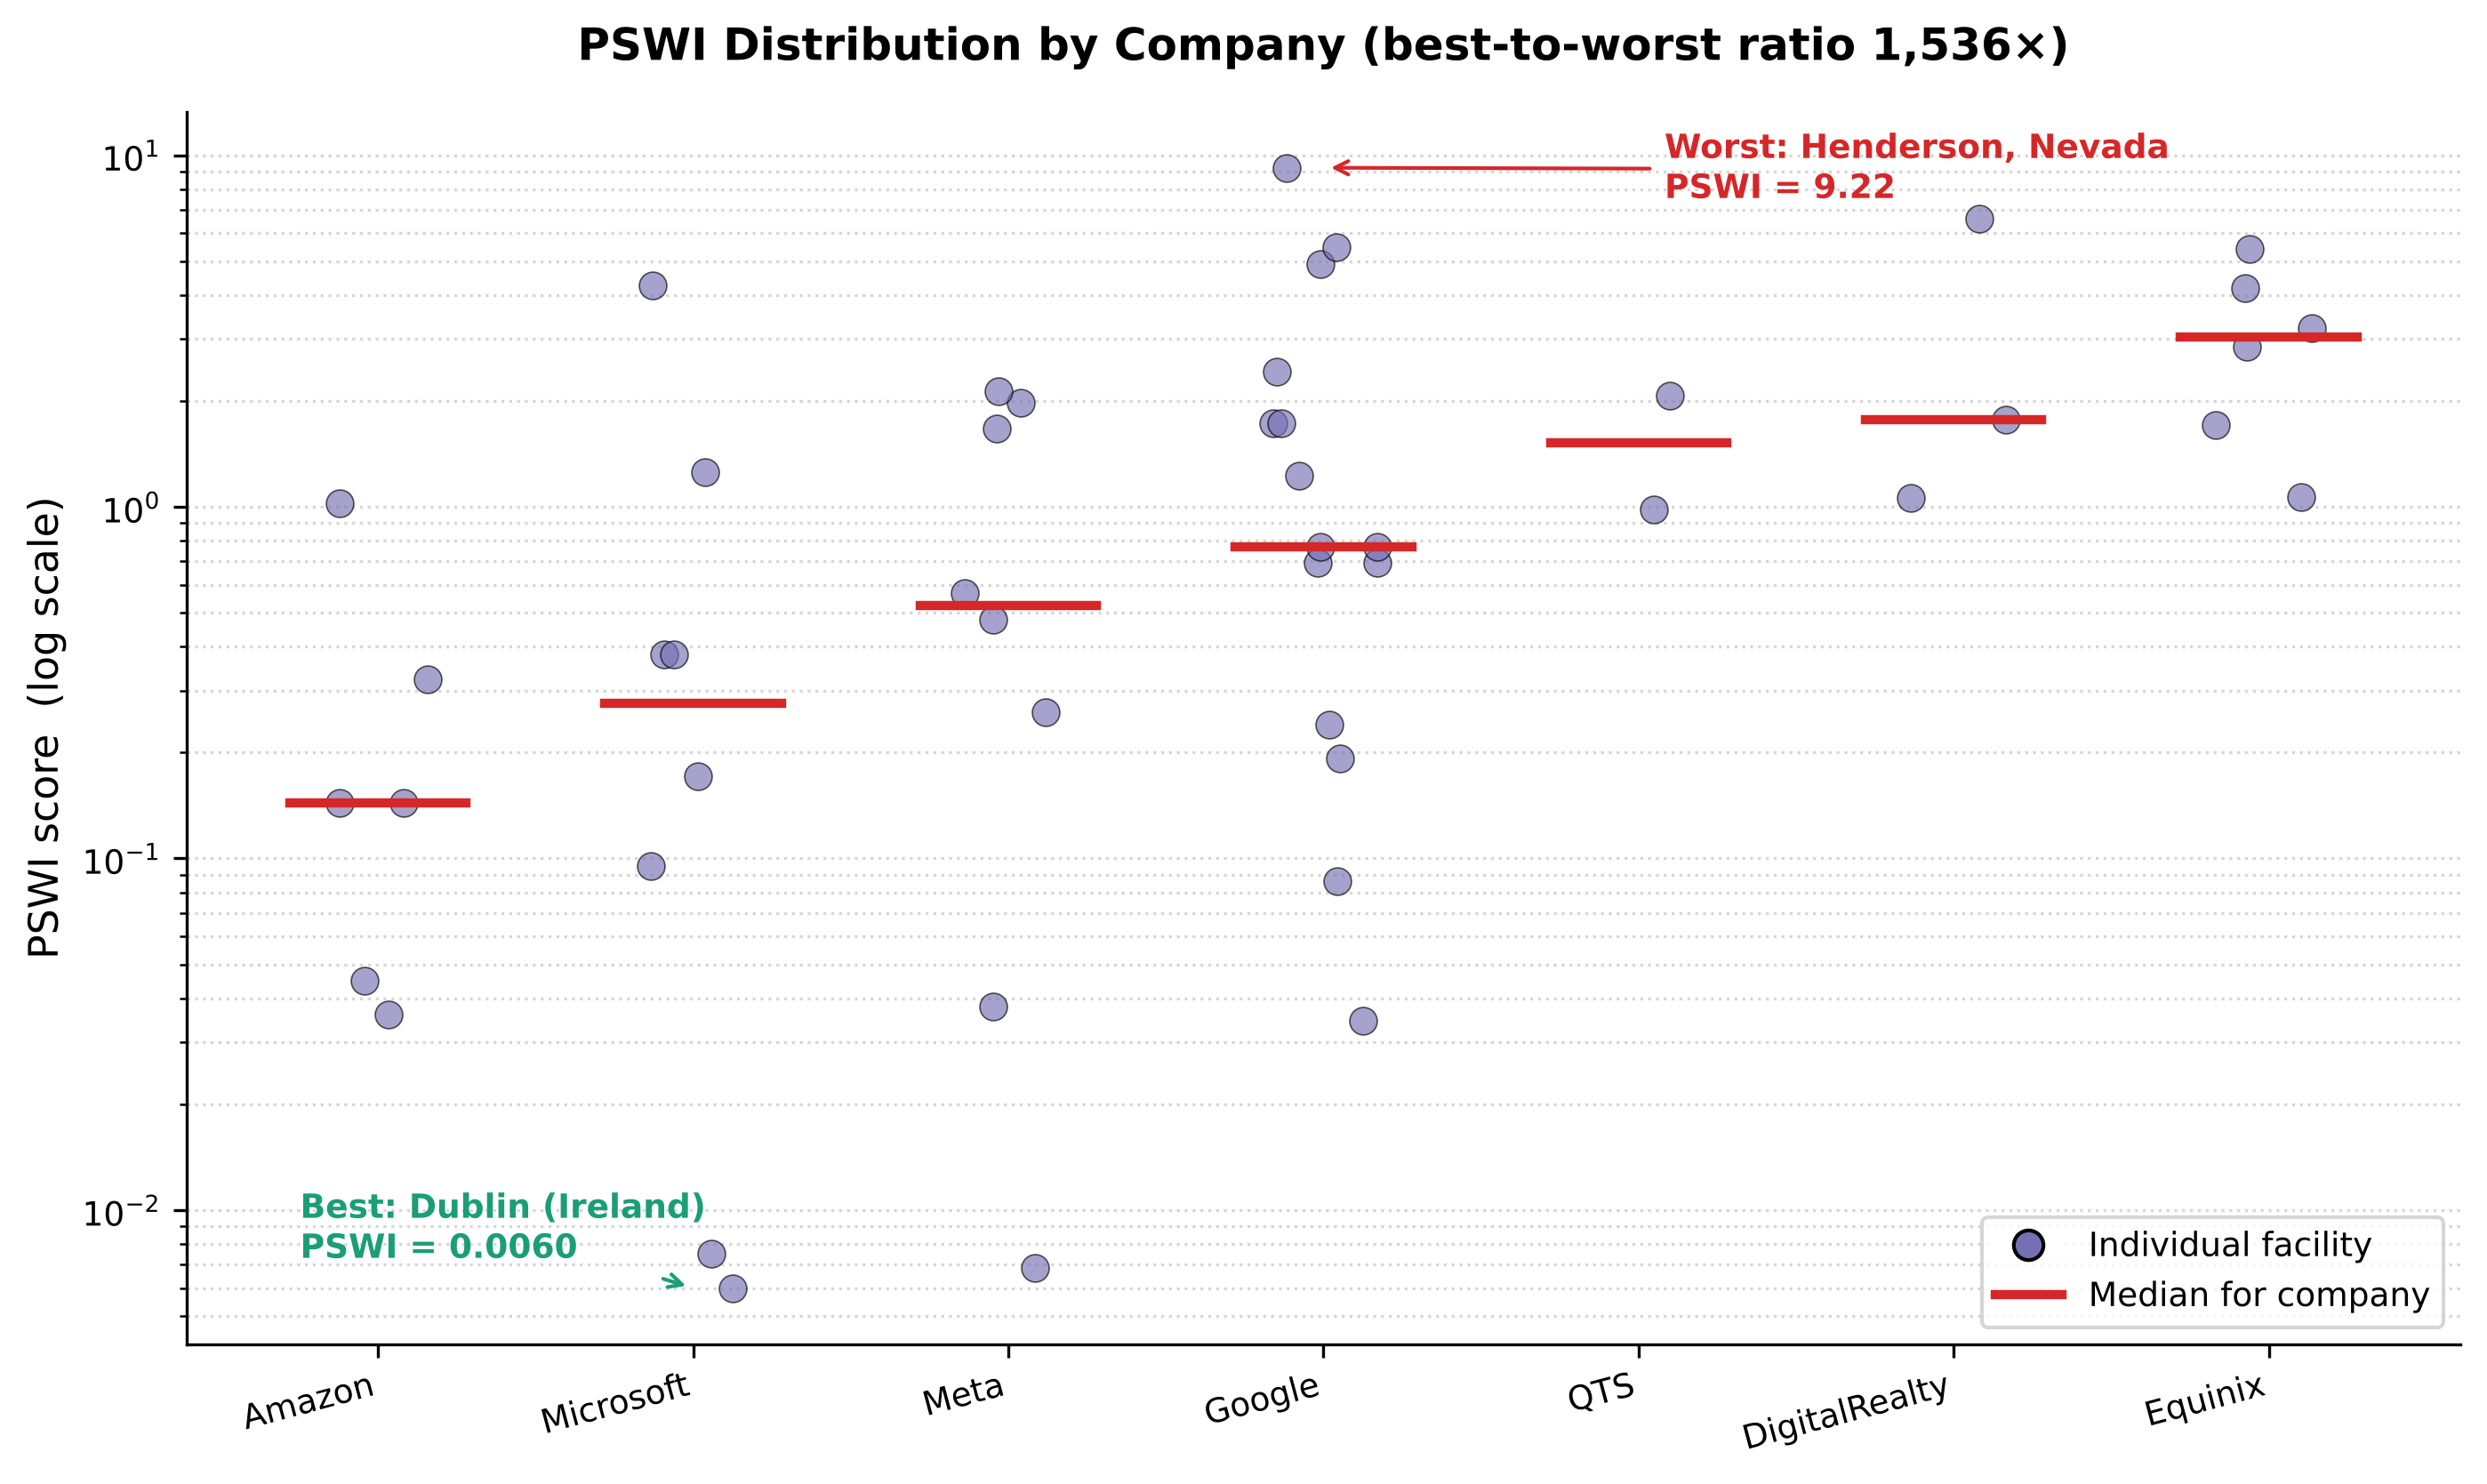
\includegraphics[width=\columnwidth]{figure_2_disparity.png}
\caption{PSWI by facility and operator (log scale). The lowest (Microsoft,
Dublin; 0.006) and highest (Google, Henderson, NV; 9.22) differ by a factor
of about 1{,}500.}
\label{fig:disparity}
\end{figure}

PSWI ranges from 0.006 (Microsoft, Dublin) to 9.22 (Google, Henderson,
Nevada), a ratio of about 1{,}500 (Fig.~\ref{fig:disparity}). The median is
0.88, with an interquartile range of 0.19 to 2.00. The range reflects both
location and the operators' differing WUE values, which span 0.03 to
0.96~L/kWh.

\subsection{Same Fleet WUE, Different PSWI}
\label{sec:samewue}

\begin{figure}[t]
\centering
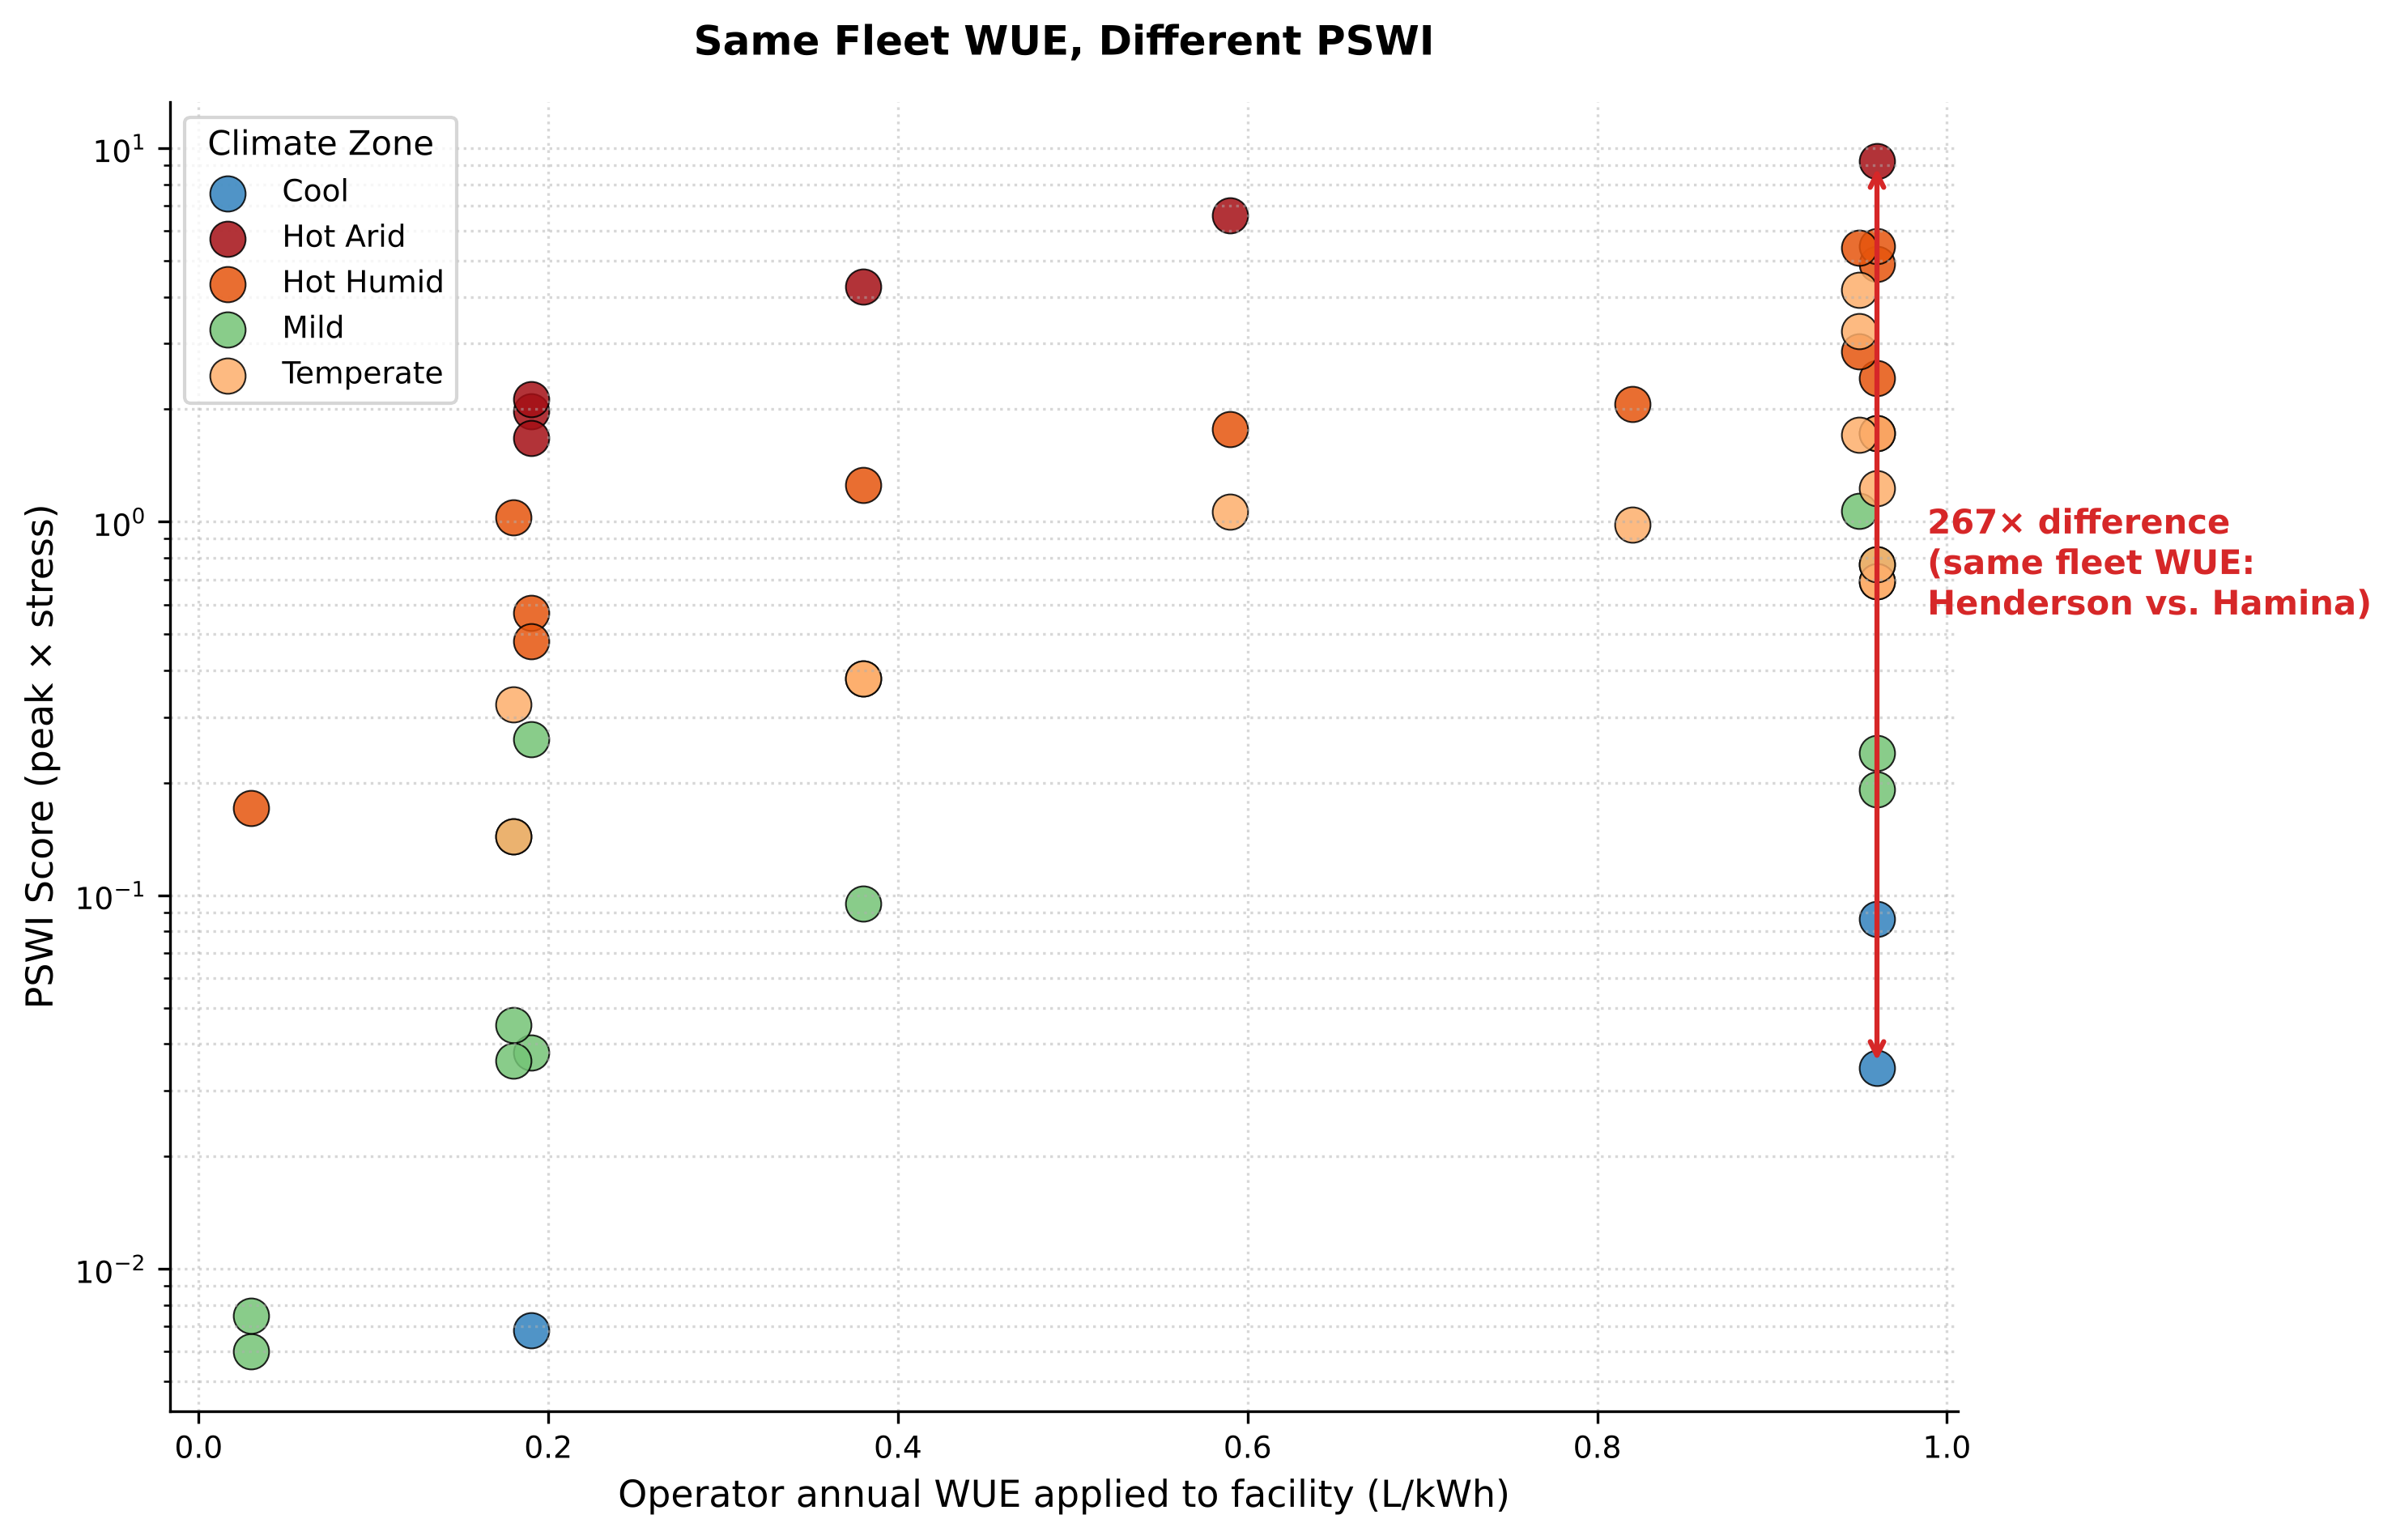
\includegraphics[width=\columnwidth]{figure_4_wue_vs_pswi.png}
\caption{PSWI versus the operator WUE applied to each facility (log
scale), colored by climate class. Vertical stacks are facilities of one
operator sharing a fleet or regional WUE. Google's Henderson and Hamina
facilities differ 267-fold at identical WUE.}
\label{fig:wuepswi}
\end{figure}

All 15 Google facilities carry the same derived fleet WUE (0.96~L/kWh), so
differences in their PSWI arise entirely from location
(Fig.~\ref{fig:wuepswi}). Henderson, Nevada ($\beta = 8.0$,
$\textrm{BWS} = 1.20$; PSWI $= 9.22$) and Hamina, Finland ($\beta = 1.8$,
$\textrm{BWS} = 0.02$; PSWI $= 0.035$) differ by a factor of 267. Of this,
a factor of 60 comes from BWS and a factor of 4.4 from the assumed peaking
factor. Lenoir, North Carolina ($\beta = 4.0$, $\textrm{BWS} = 0.18$;
PSWI $= 0.69$) and Henderson differ 13-fold. Meta's facilities, also
assigned a single fleet WUE, span a factor of 311, from Lule\aa{}, Sweden to
Mesa, Arizona.

This is not evidence about the efficiency of individual facilities, which
no operator in our sample discloses. It shows how much location-specific
burden a single fleet-level number can conceal.

\subsection{Company Rankings}

\begin{figure}[t]
\centering
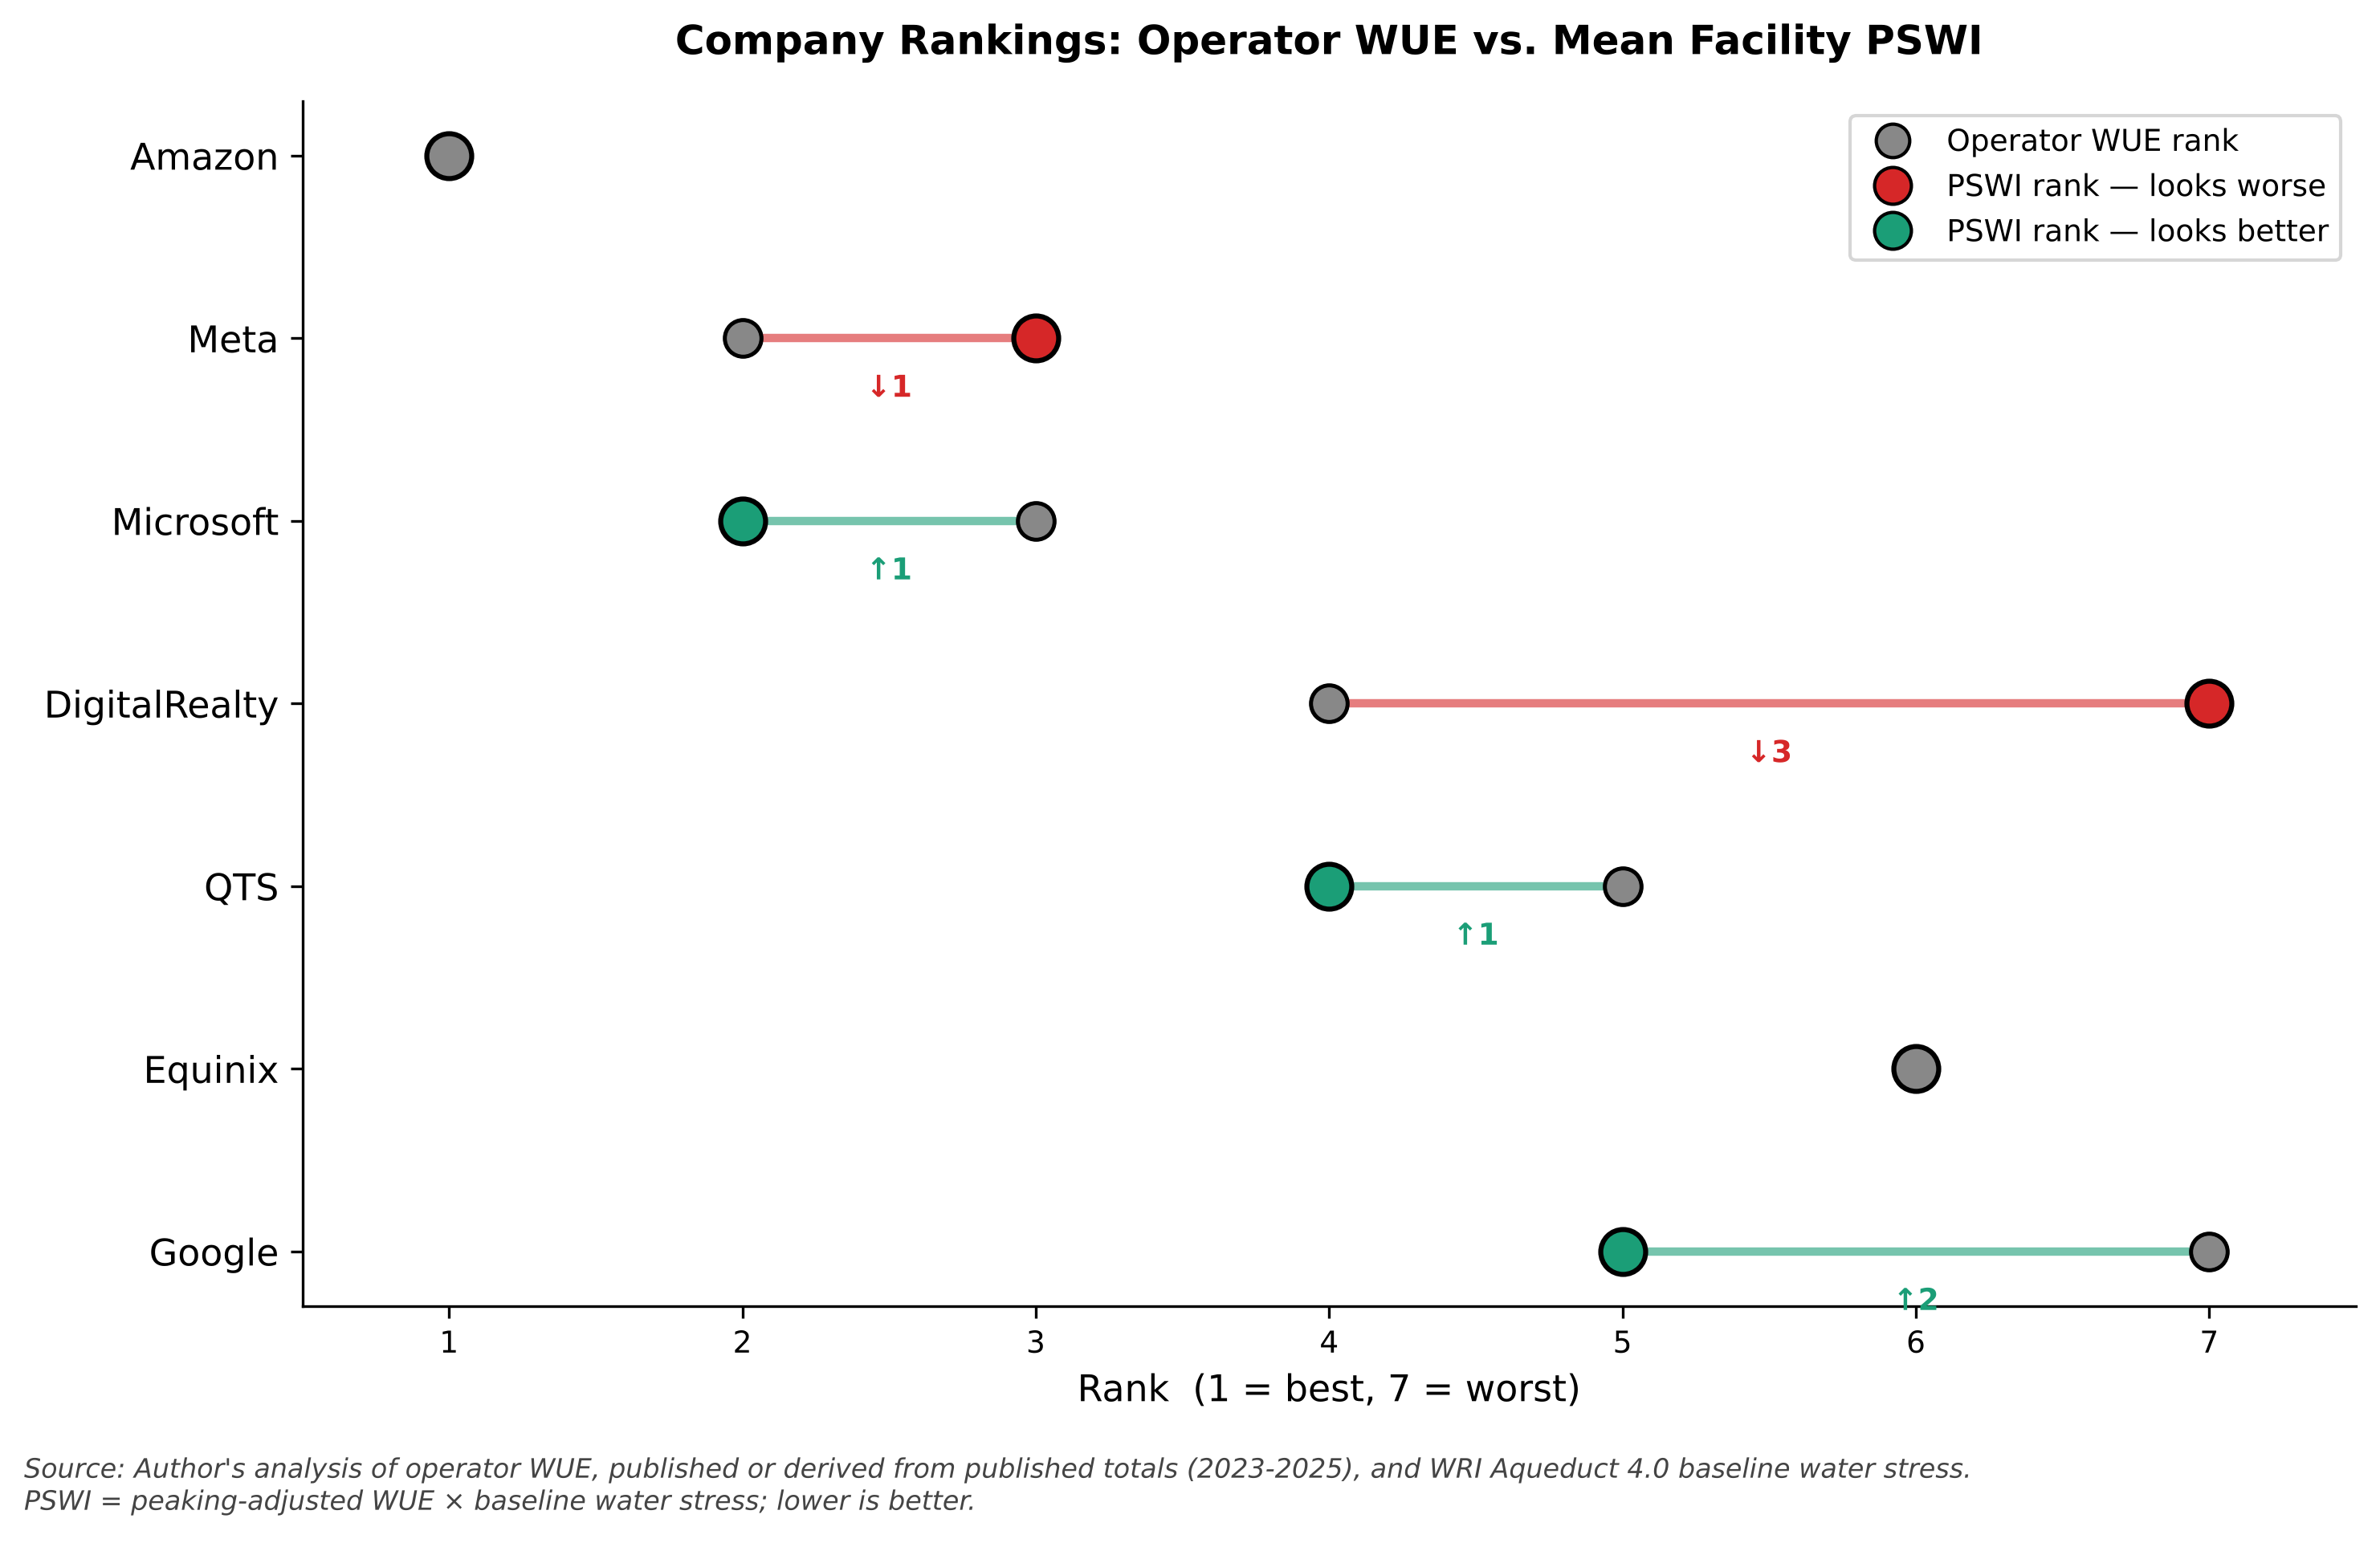
\includegraphics[width=\columnwidth]{figure_1_shell_game.png}
\caption{Company ranks by operator WUE (gray) and by unweighted mean
facility PSWI (colored). Shifts are illustrative: bootstrap intervals for
all of them include zero (Fig.~\ref{fig:bootshifts}).}
\label{fig:shellgame}
\end{figure}

\begin{figure}[t]
\centering
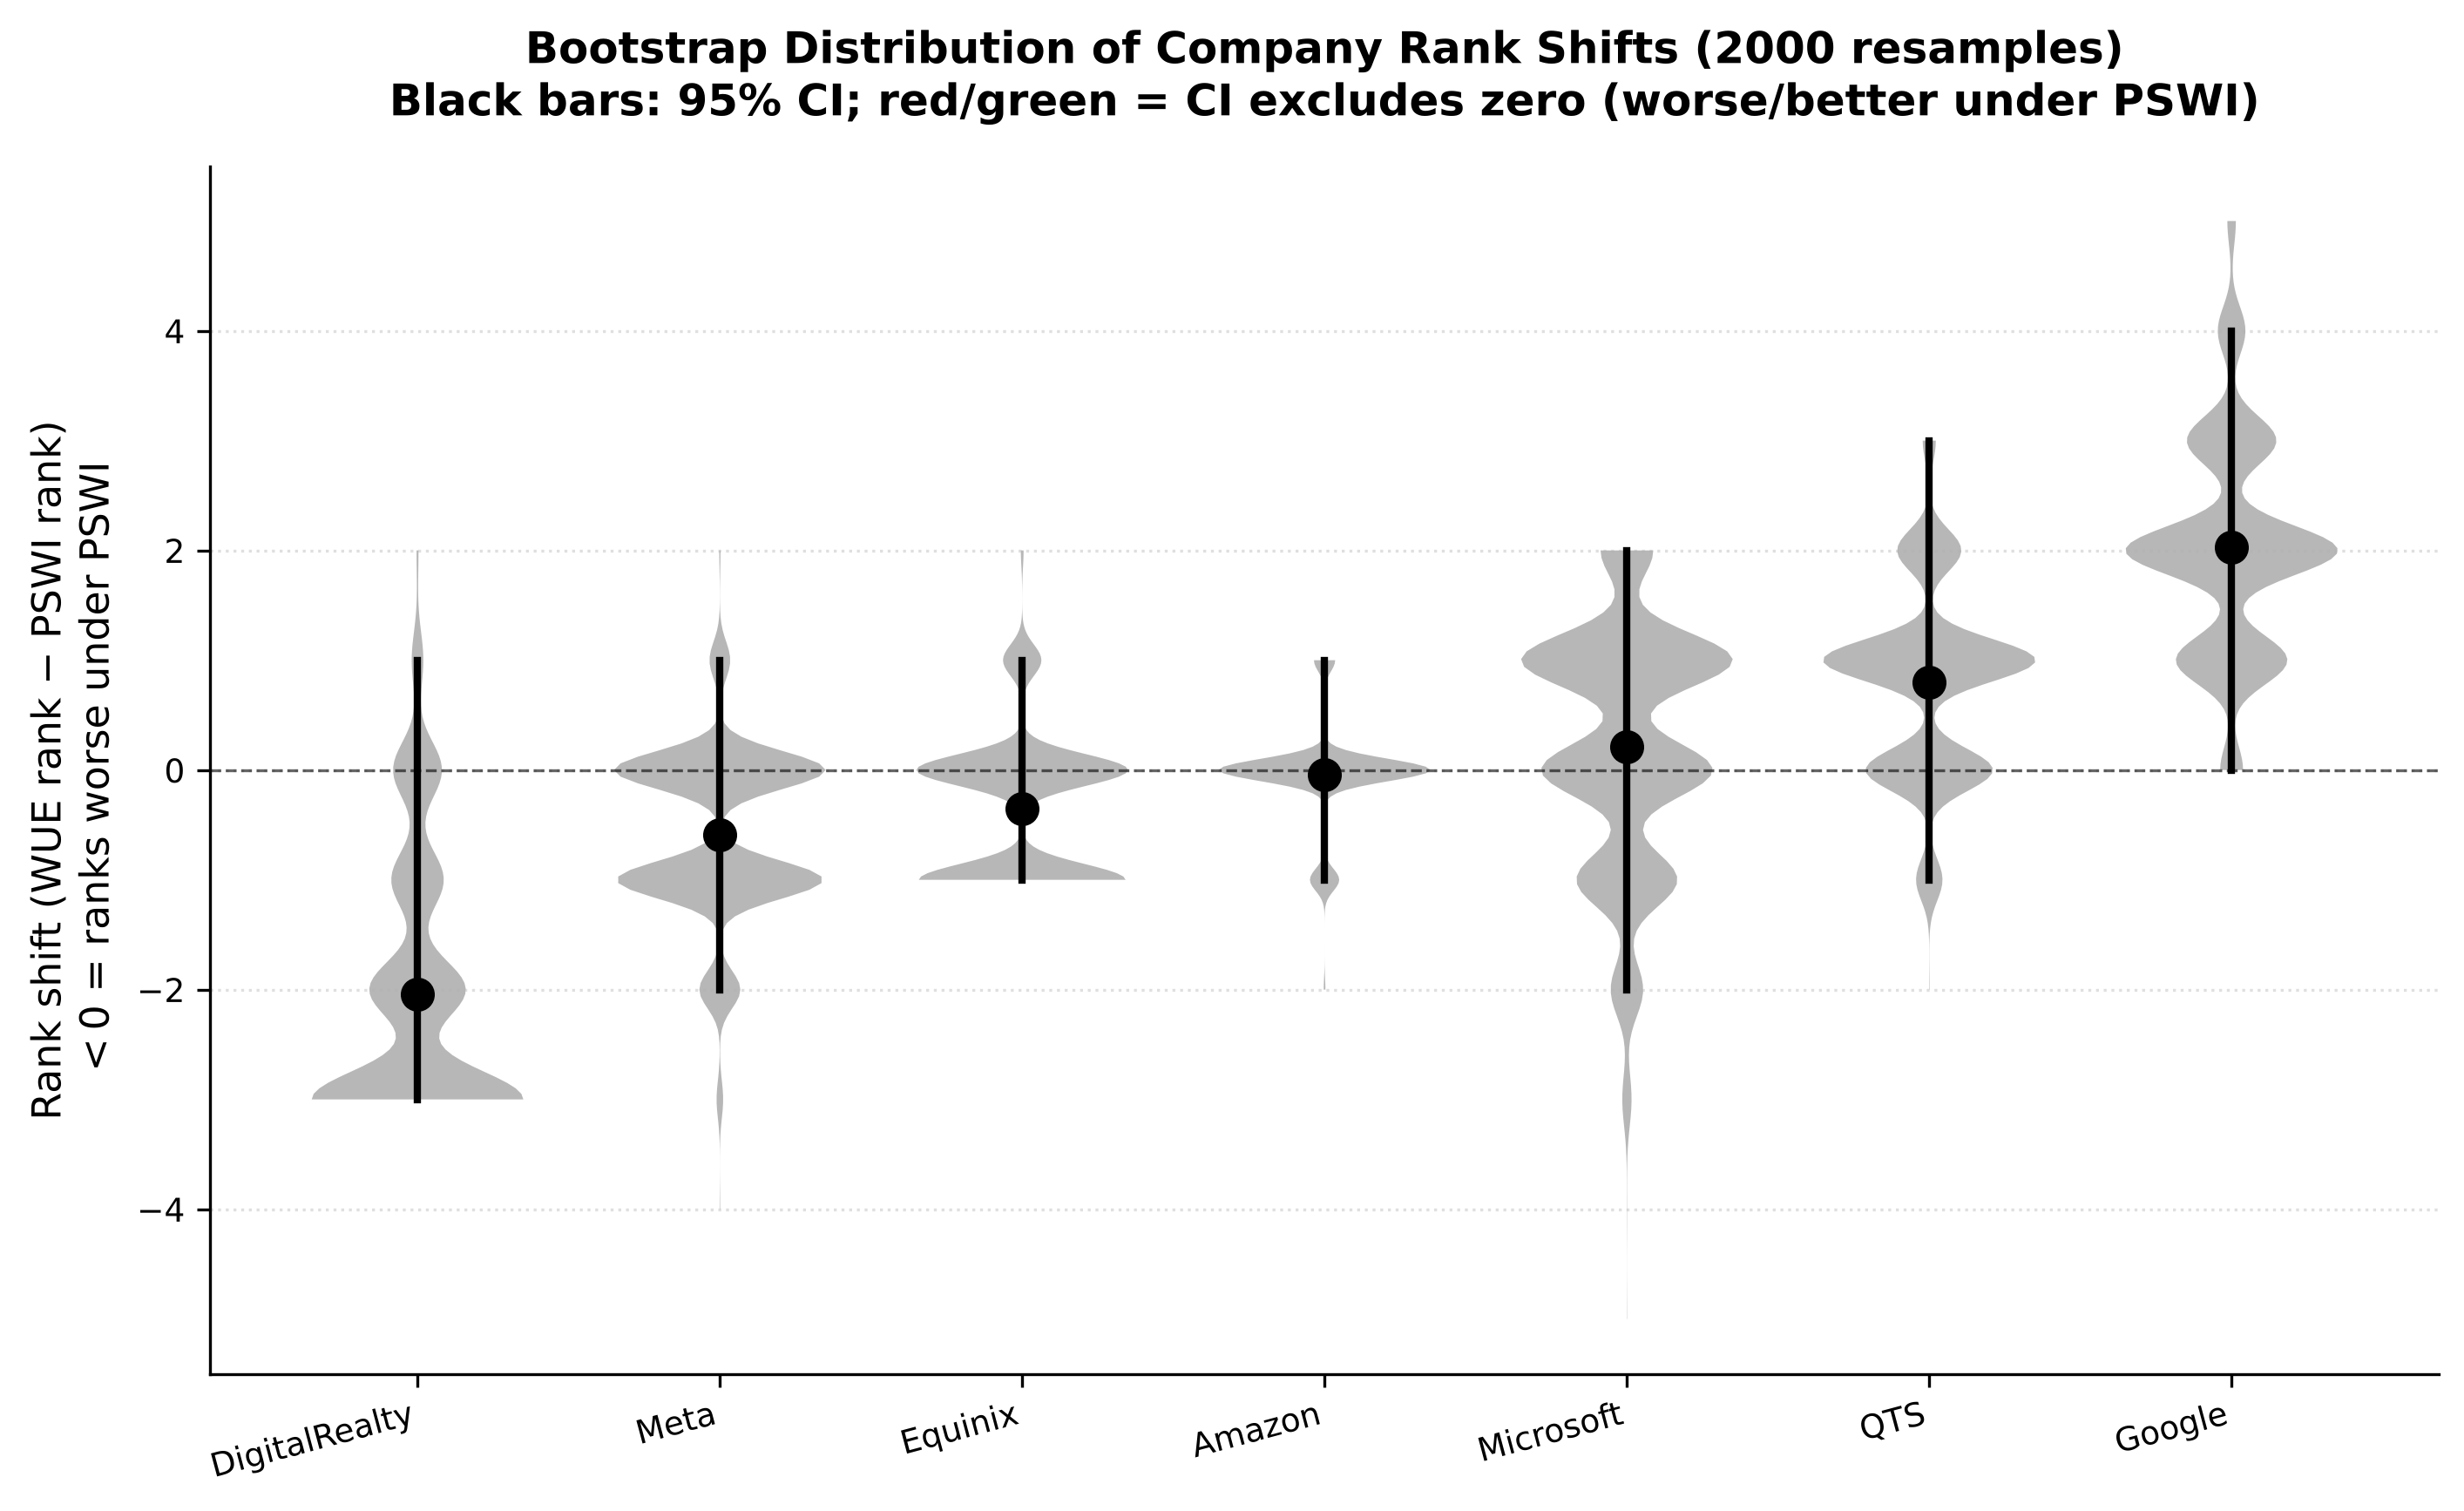
\includegraphics[width=\columnwidth]{figure_8_bootstrap_shifts.png}
\caption{Within-operator bootstrap (2{,}000 resamples) of company rank
shifts, defined as WUE rank minus PSWI rank (negative values mean a company
ranks worse under PSWI). Bars show 95\% intervals; all include zero.}
\label{fig:bootshifts}
\end{figure}

Figure~\ref{fig:shellgame} compares company ranks by operator WUE with
ranks by the unweighted mean PSWI of each company's facilities. The two
orderings are related but distinct (Spearman $\rho = 0.71$). Digital Realty
falls from fourth to seventh, driven by its Phoenix-area facility in
Chandler, Arizona (PSWI $= 6.61$). Google rises from seventh to fifth
because many of its facilities sit in low-stress catchments. Microsoft and
QTS each rise one position and Meta falls one.

A within-operator bootstrap (Fig.~\ref{fig:bootshifts}) shows that none of
these shifts is distinguishable from zero at the 95\% level (Google: mean
$+2.0$, interval $[0, +4]$; Digital Realty: mean $-2.0$, interval
$[-3, +1]$). Company means are not weighted by capacity and depend on which
facilities are sampled. We therefore treat company-level shifts as
illustrative and the facility-level results as primary.

\subsection{Variance Decomposition}

\begin{figure}[t]
\centering
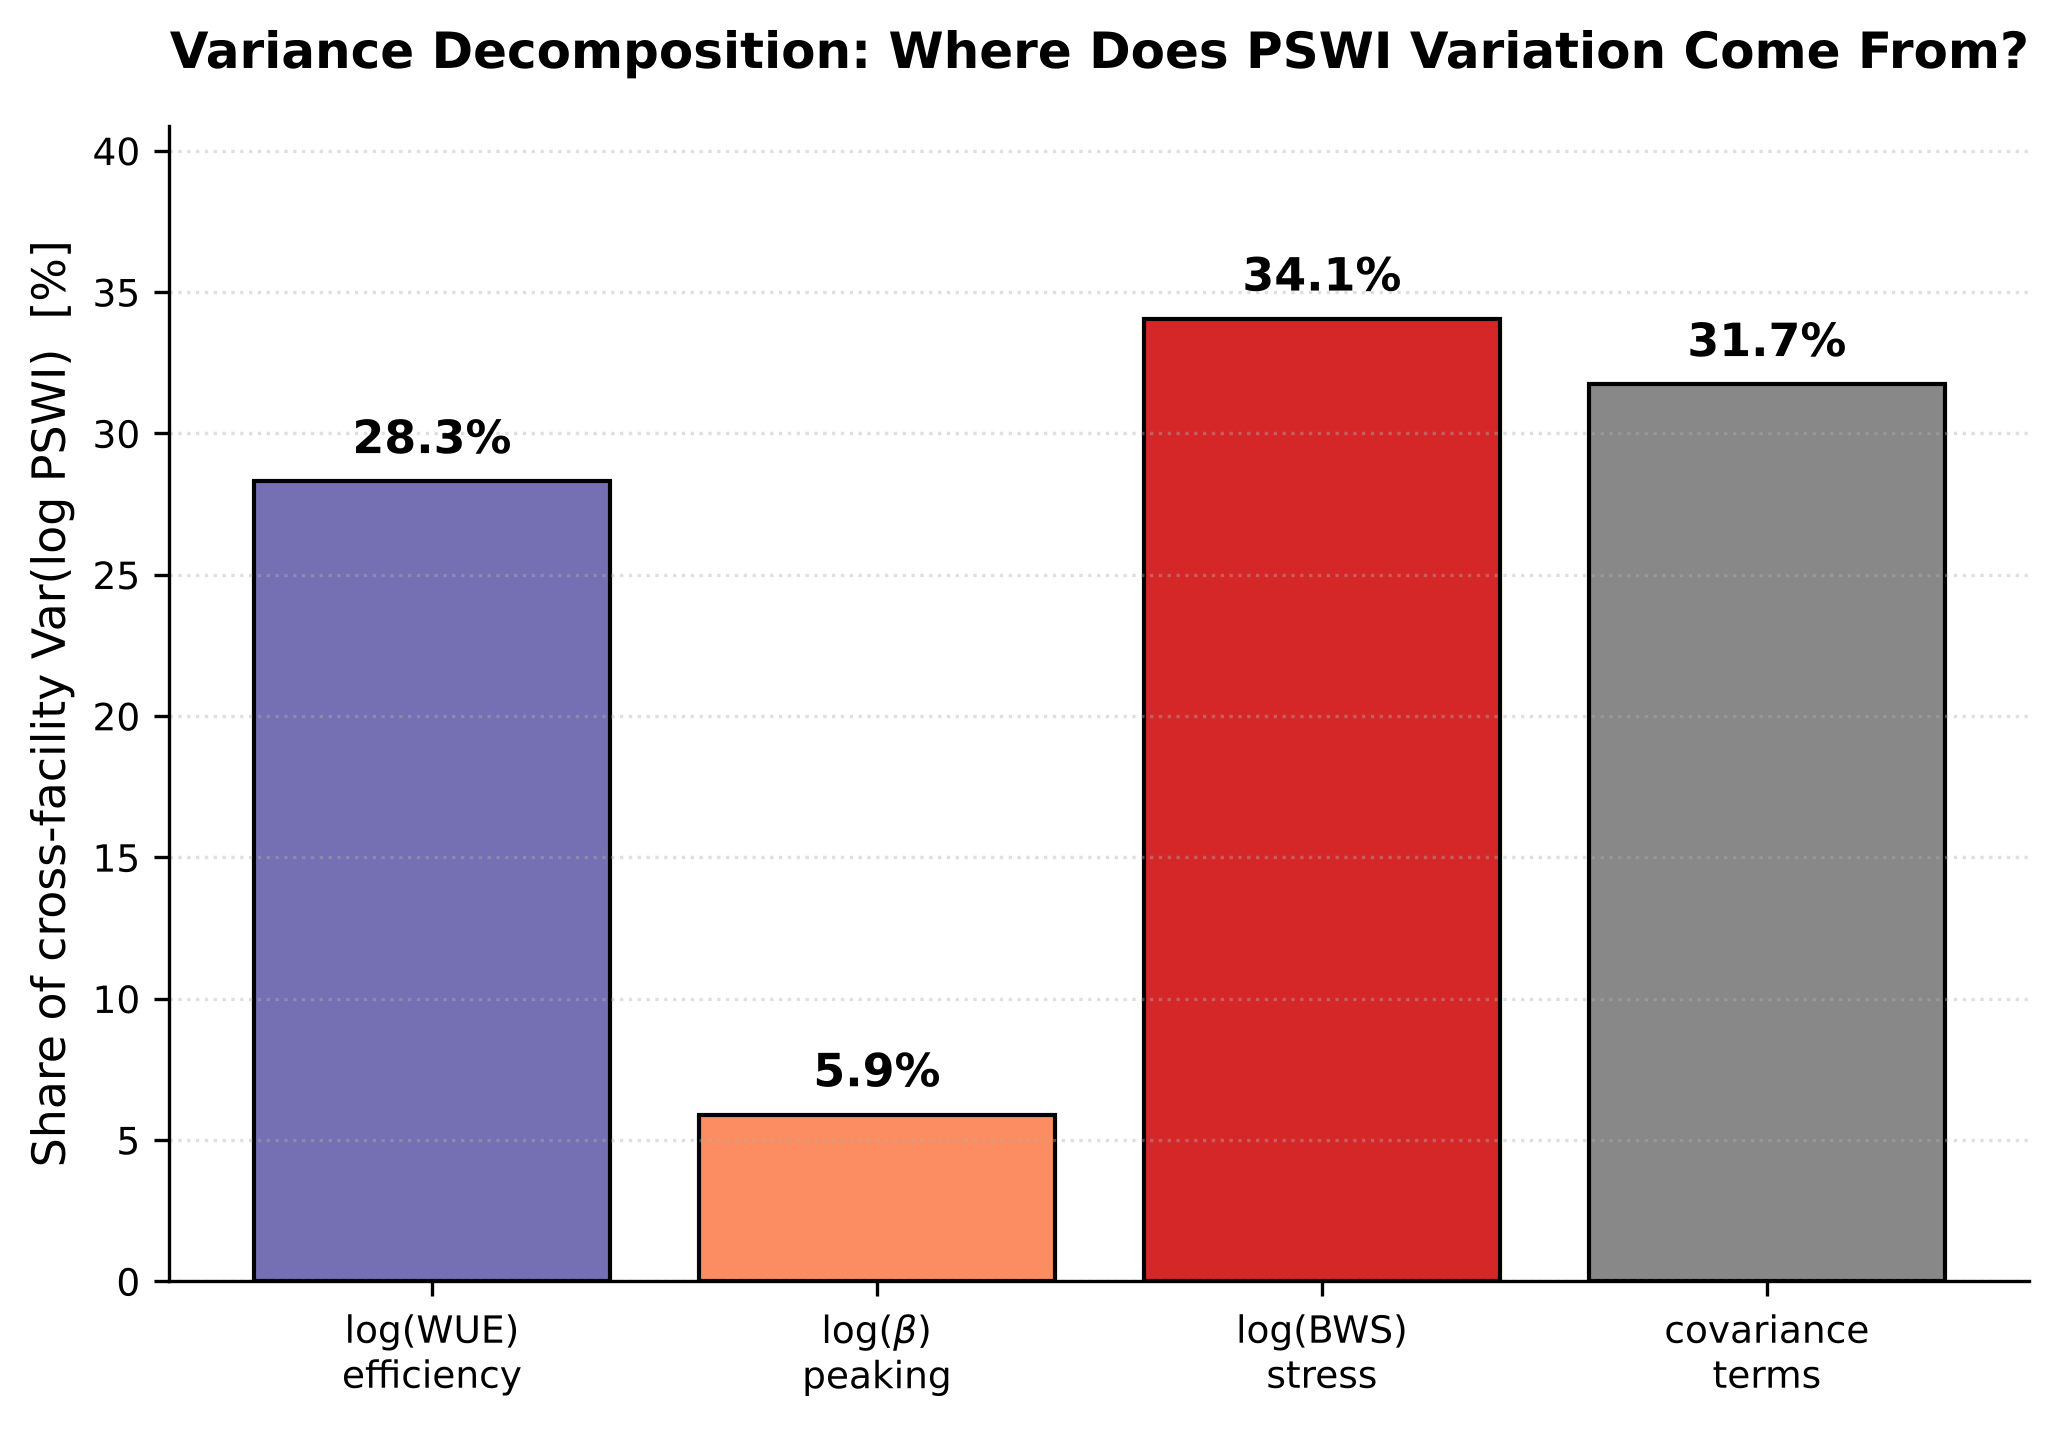
\includegraphics[width=\columnwidth]{figure_9_variance_decomposition.png}
\caption{Decomposition of $\textrm{Var}(\log\textrm{PSWI})$ across 48
facilities (Eq.~\ref{eq:vardecomp}). Most of the covariance share comes
from the $\beta$--BWS term (23.9 of 31.7 points), reflecting the
climate-based assignment of $\beta$.}
\label{fig:variance}
\end{figure}

Applying Eq.~\eqref{eq:vardecomp} across the 48 facilities
(Fig.~\ref{fig:variance}), the variance of $\log\textrm{BWS}$ accounts for
34.1\% of $\textrm{Var}(\log\textrm{PSWI})$, $\log\textrm{WUE}$ for 28.3\%,
$\log\beta$ for 5.9\%, and covariance terms for 31.7\%. Nearly all of the
covariance comes from the $\beta$--BWS pair (23.9 points; correlation 0.84
in logs), with WUE--BWS contributing 5.8 points and WUE--$\beta$ 2.0. The
$\beta$--BWS covariance is largely a consequence of assigning $\beta$ by
climate, and should not be read as independent evidence that peak demand
and stress compound. The WUE share reflects differences between operators'
published values, not differences between facilities of one operator.

\subsection{Sensitivity to the Peaking Factor}
\label{sec:betasens}

\begin{figure*}[t]
\centering
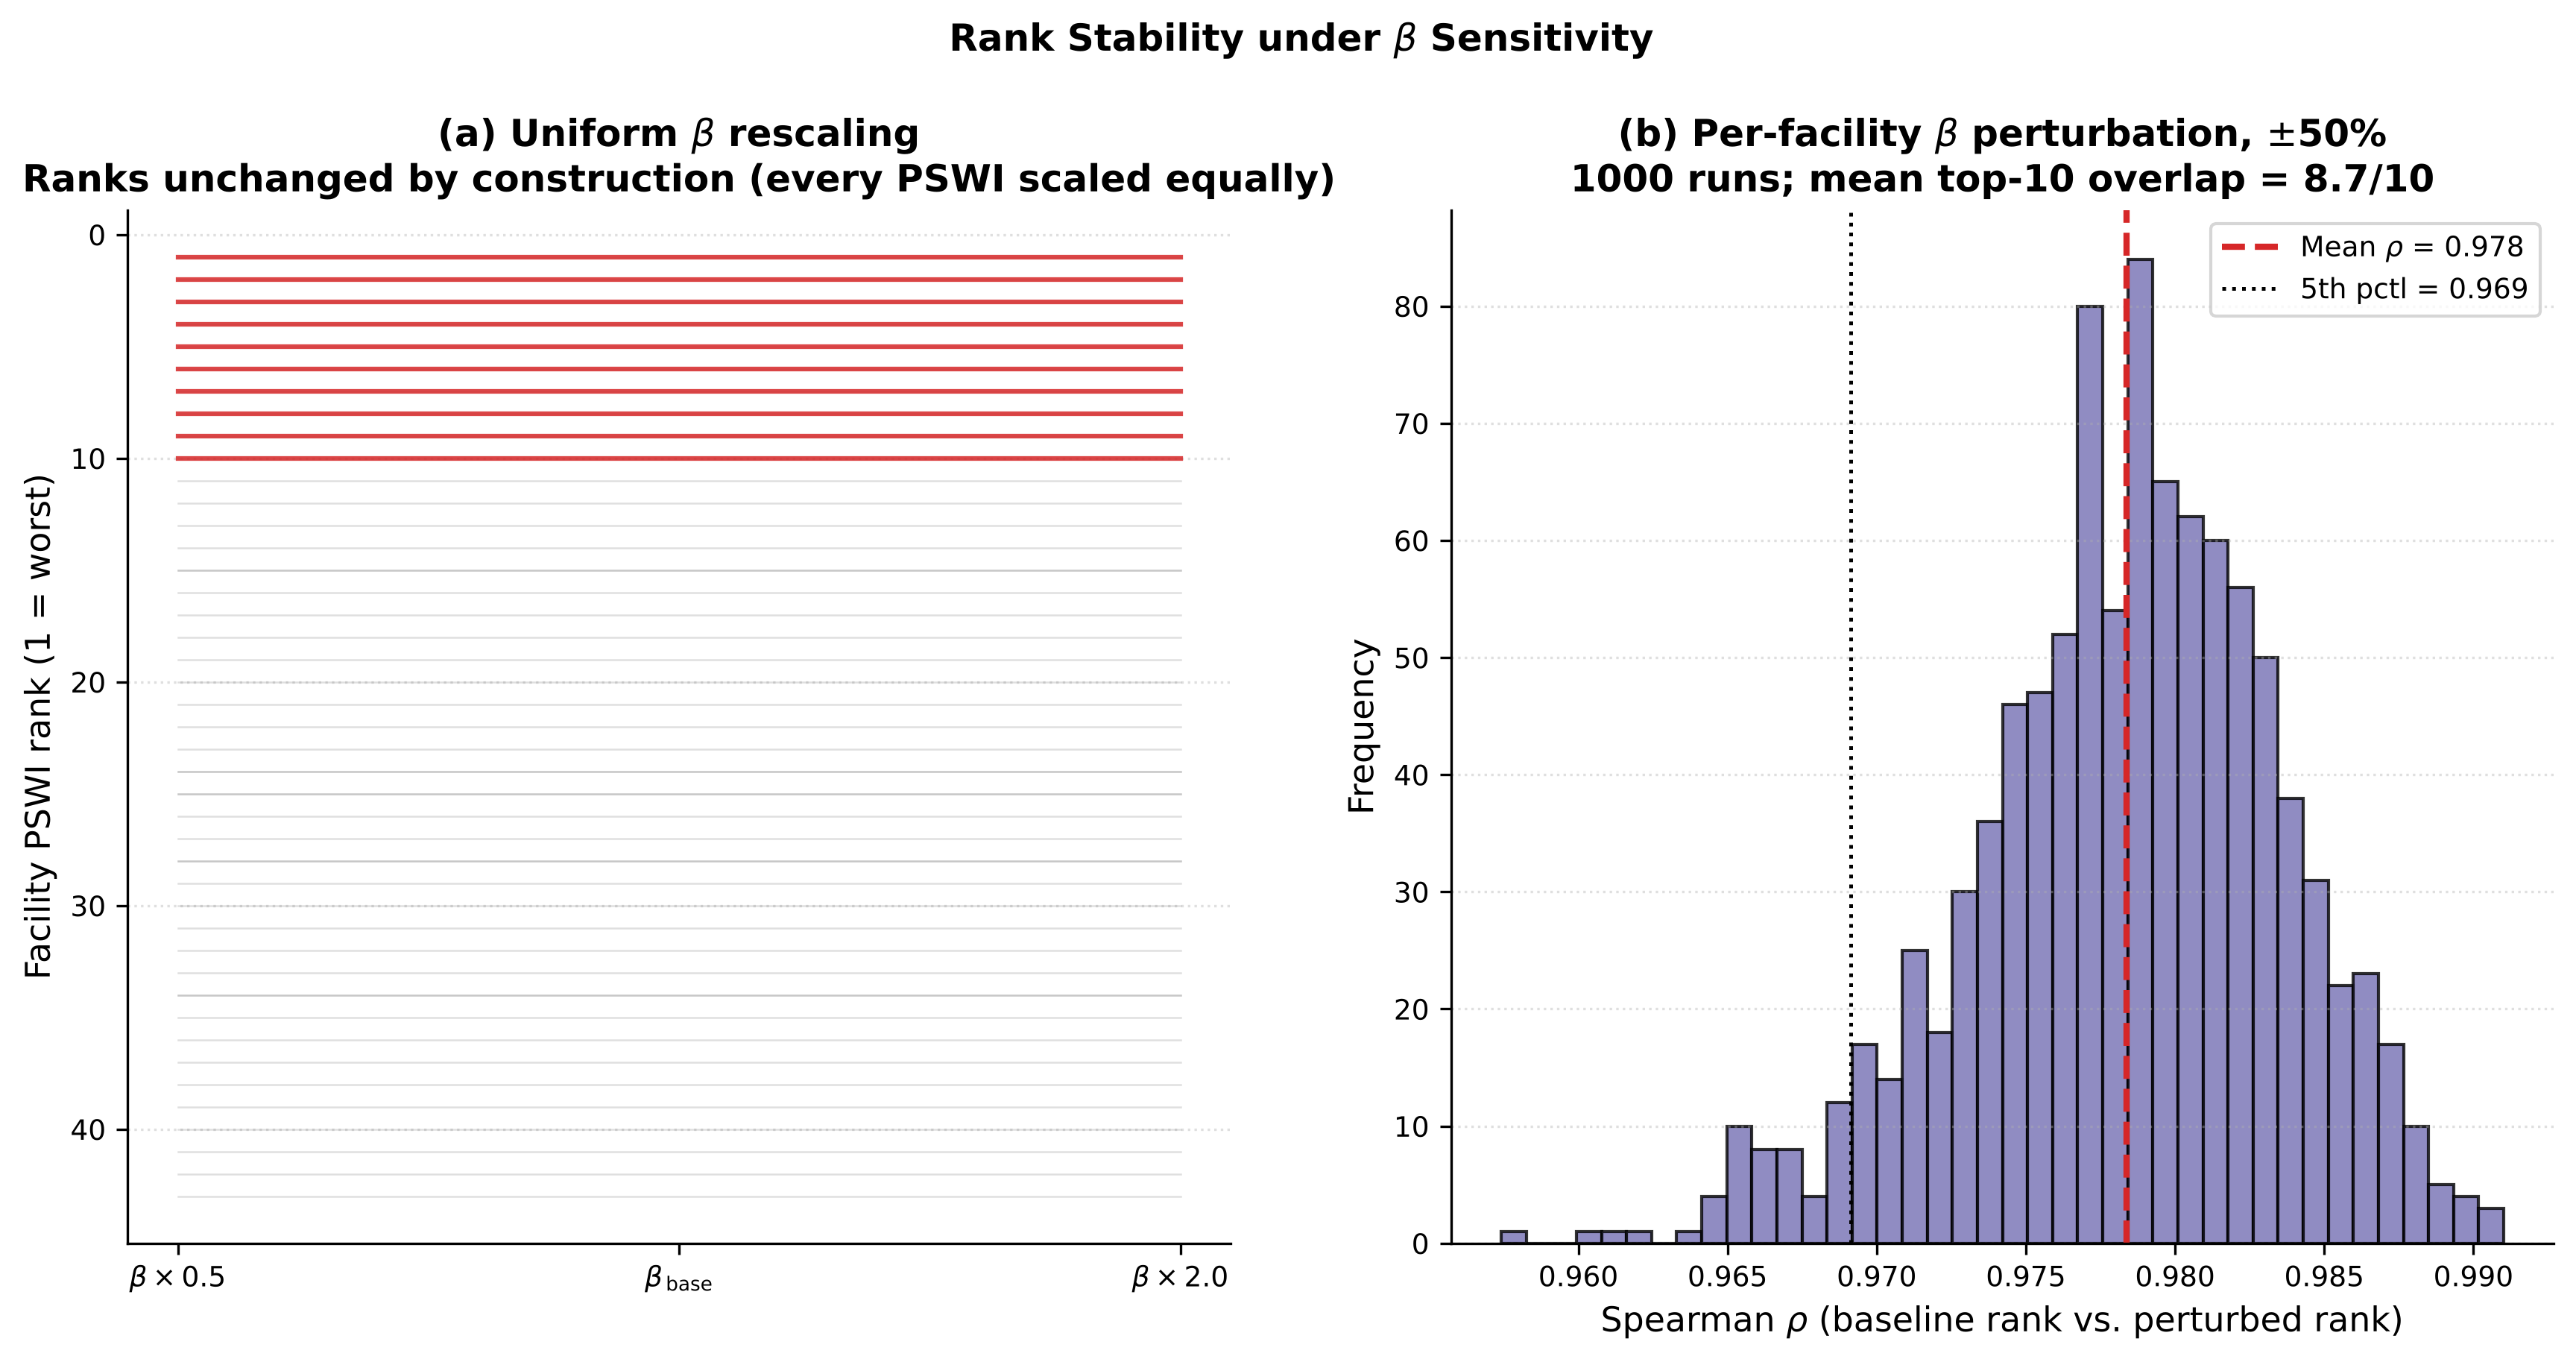
\includegraphics[width=0.82\textwidth]{figure_7_beta_sensitivity.png}
\caption{(a) Uniform rescaling of $\beta$ leaves ranks unchanged by
construction. (b) Independent per-facility perturbation of $\beta$ by up to
$\pm$50\% (1{,}000 runs): mean Spearman $\rho = 0.978$ between baseline and
perturbed facility rankings.}
\label{fig:beta}
\end{figure*}

\begin{figure}[t]
\centering
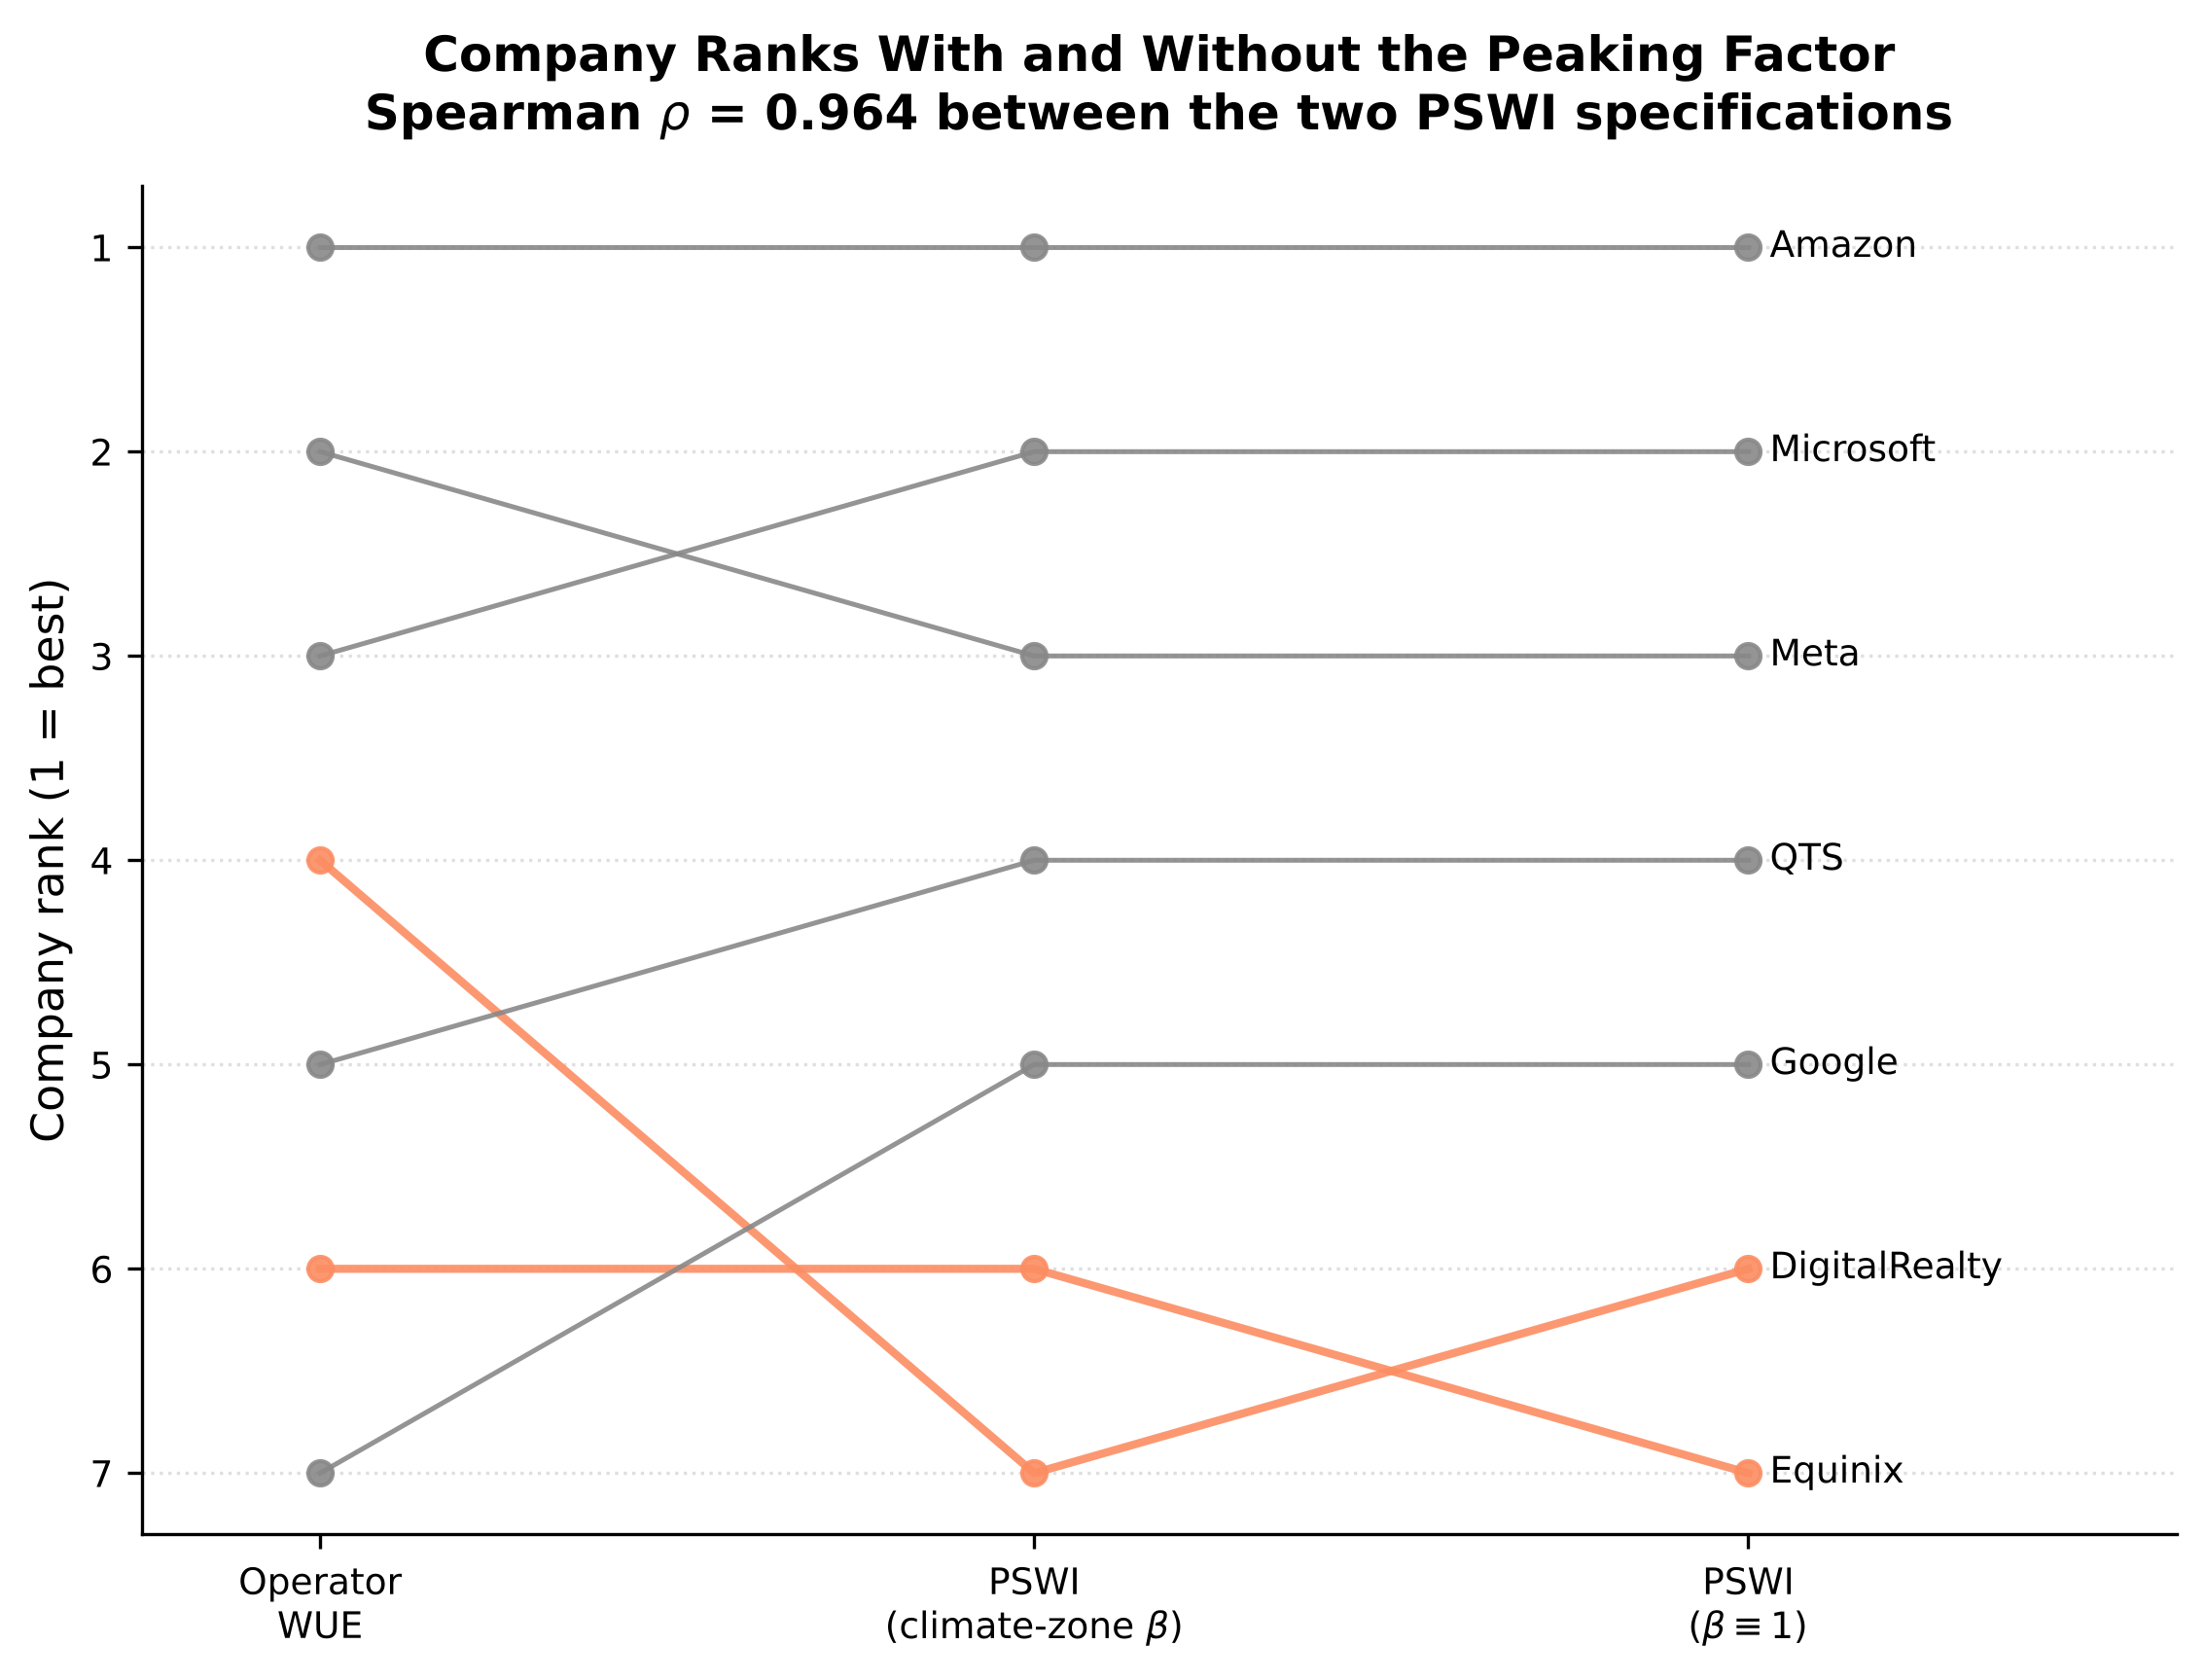
\includegraphics[width=\columnwidth]{figure_11_beta_null.png}
\caption{Company ranks under operator WUE, PSWI with climate-class
$\beta$, and PSWI with $\beta \equiv 1$. Rankings under the two PSWI
specifications correlate at $\rho = 0.964$.}
\label{fig:betanull}
\end{figure}

Uniform rescaling of the $\beta$ table leaves rankings unchanged by
construction (Fig.~\ref{fig:beta}a). Independent per-facility perturbations
of $\beta$ drawn uniformly within $\pm$50\% (1{,}000 runs) give a mean
Spearman $\rho$ of 0.978 between baseline and perturbed facility rankings
(5th percentile 0.969), and retain on average 8.7 of the 10 highest-PSWI
facilities (Fig.~\ref{fig:beta}b).

The stricter test removes the peaking factor entirely ($\beta \equiv 1$, so
that $\textrm{PSWI} \propto \textrm{WUE} \cdot \textrm{BWS}$). Facility
rankings then correlate at $\rho = 0.963$ with the main specification, and
9 of the 10 highest-PSWI facilities are unchanged. Company rankings
correlate at $\rho = 0.964$, and no company's shift changes direction
(Fig.~\ref{fig:betanull}). The peaking factor thus adds the peak-demand
dimension to the magnitude of PSWI but has little effect on rankings in
this sample, which are driven mainly by BWS. Measured, facility-specific
peaking factors could change this.

\subsection{Scope 2 Sensitivity}
\label{sec:scope2}

To test whether omitting indirect water changes the picture, we add
3.14~L/kWh, the U.S.\ average electricity water-consumption intensity used
by Li et al.~\cite{li2023thirsty}, to every facility's WUE before applying
$\beta$ and BWS. Facility rankings correlate at $\rho = 0.88$ with the main
specification, 6 of the 10 highest-PSWI facilities are retained, and the
mean absolute rank change is 5.2 positions. This is a crude stress test:
Scope~2 water is drawn at power plants, often in other basins with
different peaking behavior, and a U.S.\ average is applied to non-U.S.\
sites. A proper treatment would weight indirect water by the stress of the
generating basin, as AWI does~\cite{wu2025scarf}.

\subsection{Geographic Concentration}

\begin{figure*}[t]
\centering
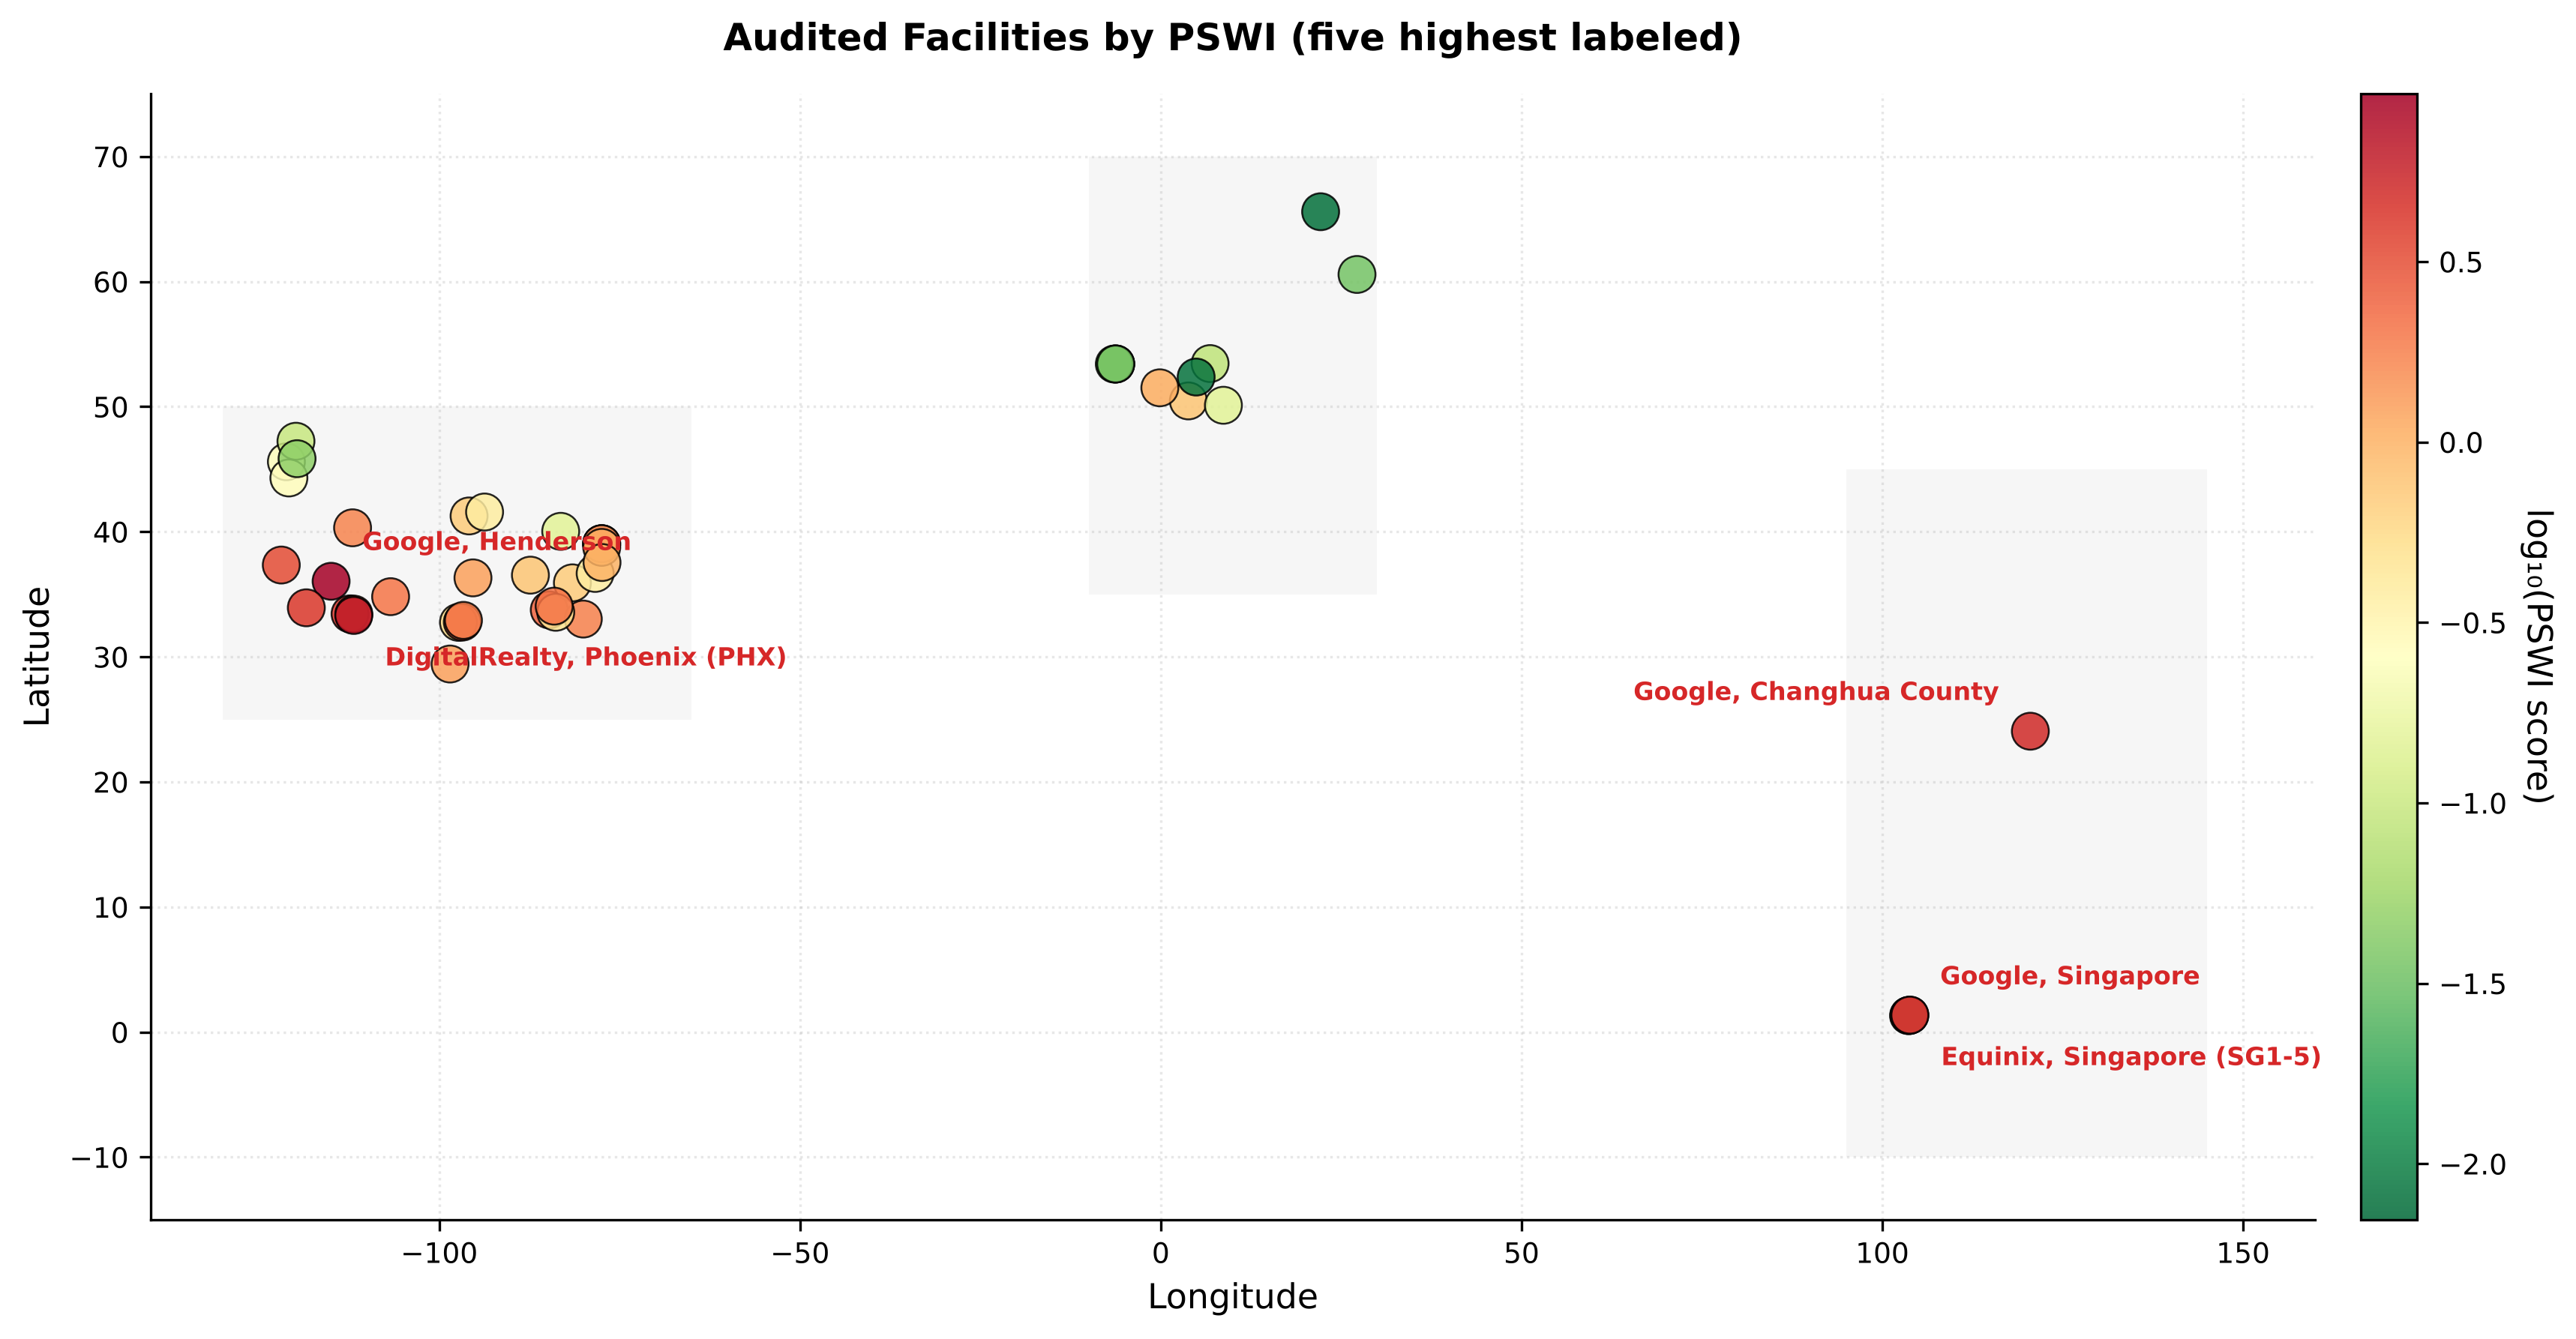
\includegraphics[width=0.85\textwidth]{figure_3_world_map.png}
\caption{Audited facilities colored by $\log_{10}(\textrm{PSWI})$; the five
highest are labeled. High values cluster in the U.S.\ West and in Singapore
and Taiwan; Northern and Western Europe are low.}
\label{fig:map}
\end{figure*}

Of the 10 highest-PSWI facilities (Fig.~\ref{fig:map}), five are in the
U.S.\ West (Henderson, Nevada; Chandler and Goodyear, Arizona; El Segundo
and San Jose, California), three are in Singapore and Taiwan, and two are
in Texas and Georgia. Of the 10 lowest, seven are in Northern and Western
Europe (Hamina, Finland; Lule\aa{}, Sweden; Eemshaven and Amsterdam,
Netherlands; and three in the Dublin area), two are in the U.S.\ Pacific
Northwest (Boardman, Oregon; Quincy, Washington), and one is in Ohio.
Several high-PSWI locations are established data center markets, so siting
decisions there carry disproportionate water-stress consequences.

\subsection{Disclosure Audit}
\label{sec:disclosure}

\begin{figure}[t]
\centering
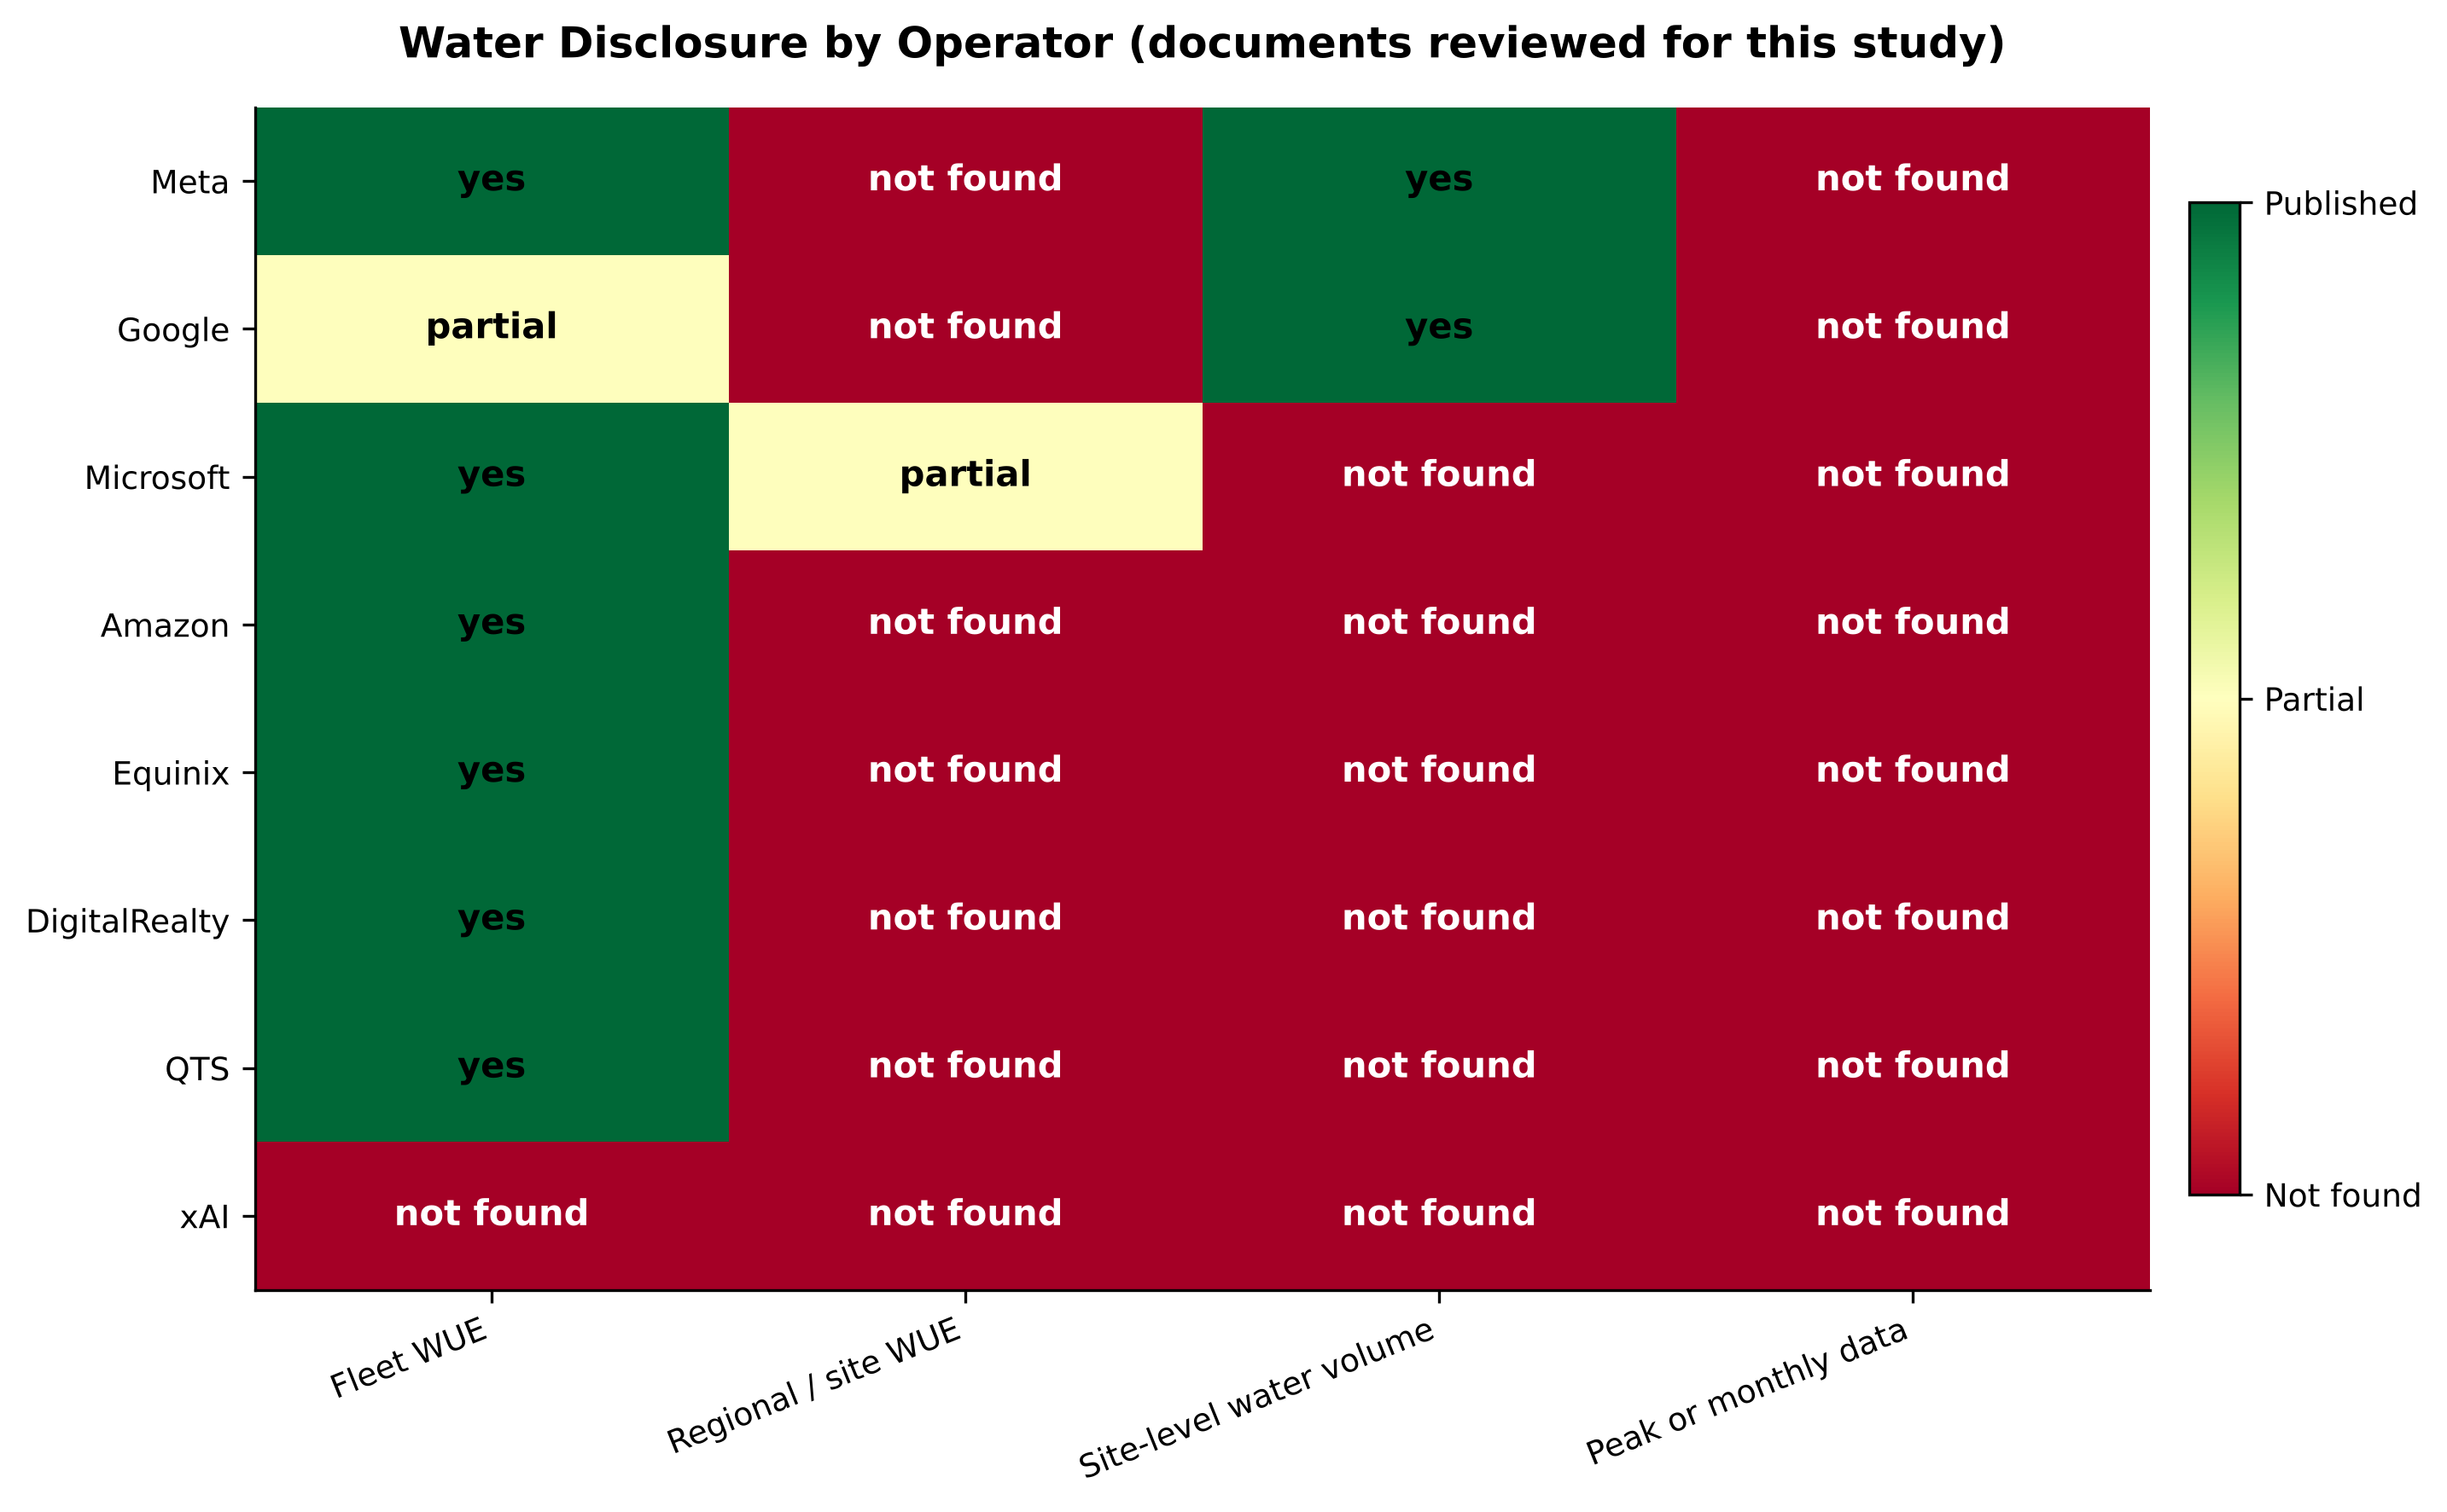
\includegraphics[width=\columnwidth]{figure_6_disclosure.png}
\caption{Water disclosure by operator in the documents reviewed for this
study. ``Not found'' means absent from those documents. No operator
publishes peak or monthly water data.}
\label{fig:disclosure}
\end{figure}

Figure~\ref{fig:disclosure} summarizes what the documents cited in our
dataset disclose for each operator, with xAI shown for reference. Six of the
seven sampled operators publish a fleet-level WUE; Google does not, although
one can be derived from its published totals. Only Microsoft publishes WUE
below the fleet level, and only by region. Google and Meta publish
facility-level water volumes but not the facility energy needed to compute
WUE. We found no peak-day or monthly water data from any operator, and no
WUE from xAI. Because no operator publishes facility-level WUE or peak data,
no outside party can compute a fully facility-specific PSWI for any
facility in our sample.

% ============================================================================
\section{Counterfactual Analysis and Policy Implications}
\label{sec:policy}
% ============================================================================

\subsection{Idealized Reallocation Counterfactual}

\begin{figure}[t]
\centering
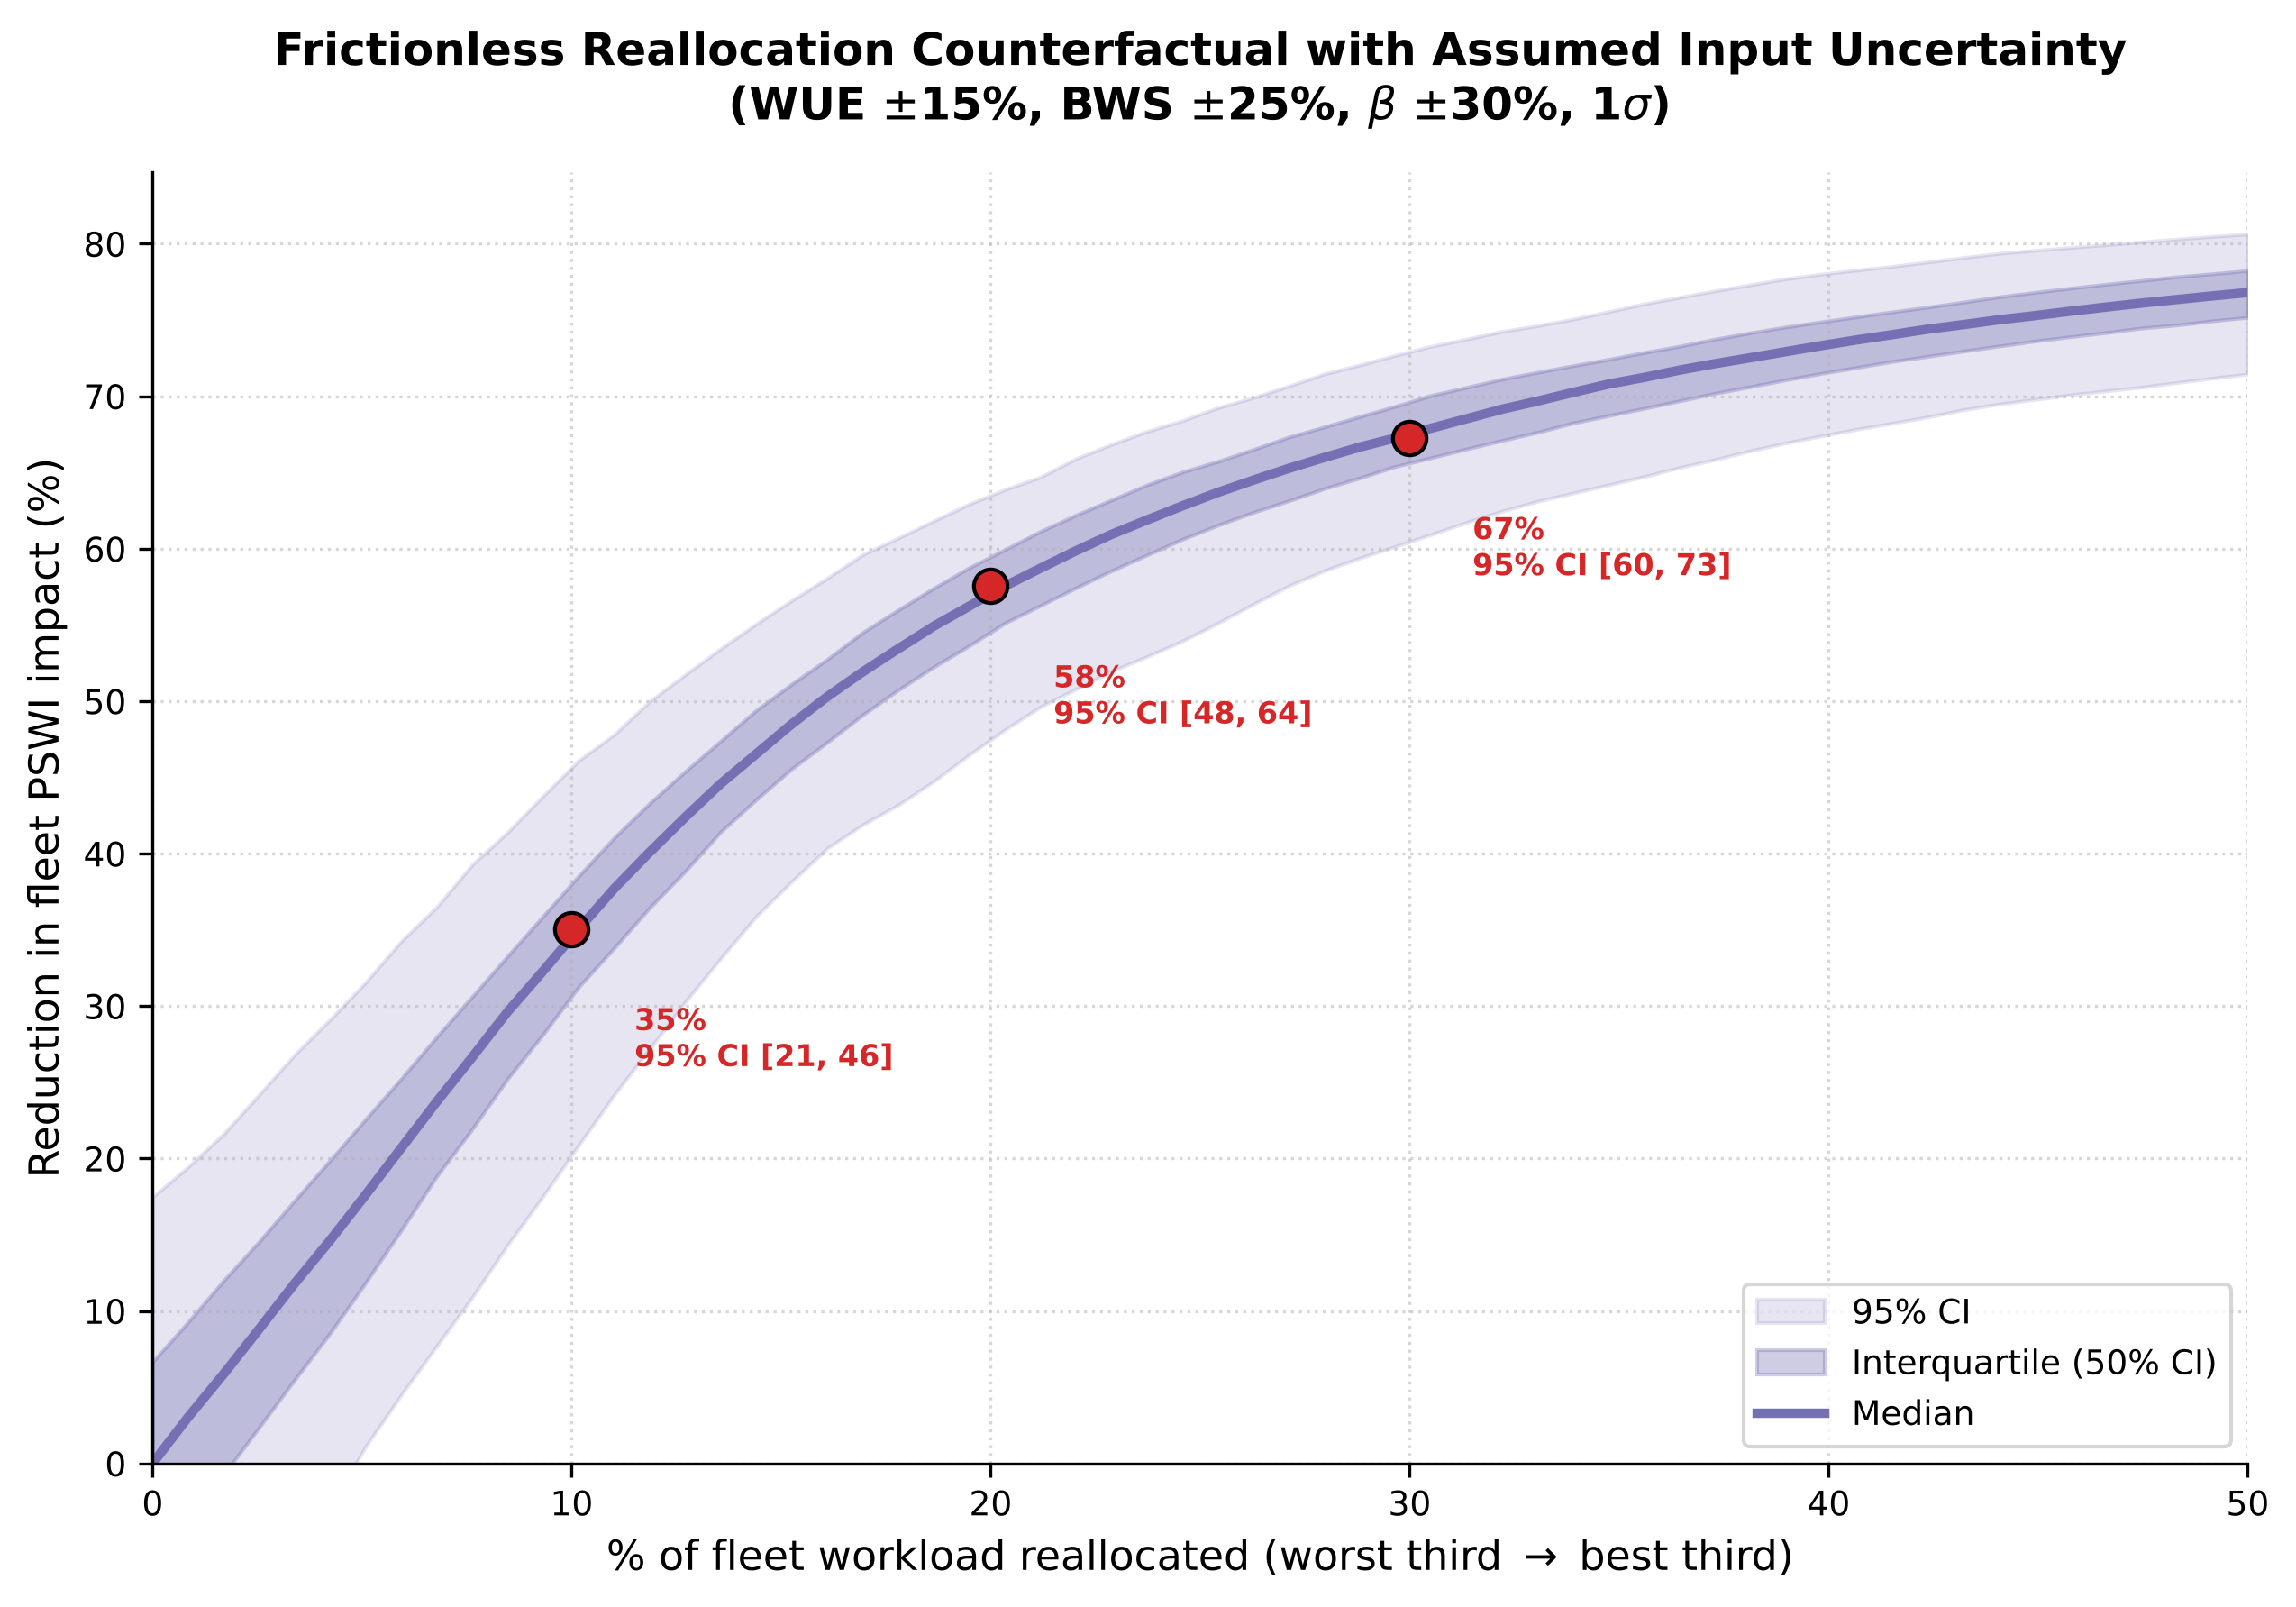
\includegraphics[width=\columnwidth]{figure_10_counterfactual_uncertain.png}
\caption{Idealized, frictionless reallocation from the highest- to the
lowest-PSWI third of facilities with assumed input uncertainty (WUE
$\pm$15\%, BWS $\pm$25\%, $\beta$ $\pm$30\%, 1$\sigma$; 500 runs). At 10\%
reallocation the median reduction in aggregate PSWI is 35\% (95\% interval
21--46\%).}
\label{fig:counterfactual}
\end{figure}

\paragraph{Setup}
Each facility starts with a workload of one unit. A fraction $f$ of total
workload is removed from the highest-PSWI third of facilities, in
proportion to their PSWI, and reassigned to the lowest-PSWI third, in
inverse proportion to their PSWI. In each of 500 Monte Carlo draws, WUE,
BWS, and $\beta$ are perturbed independently by normal relative errors with
standard deviations of 15\%, 25\%, and 30\% ($\beta$ floored at 1). These
uncertainty levels are assumptions chosen to be generous, not estimates
from a published error model.

\paragraph{Results}
At $f \approx 10\%$, aggregate PSWI falls by a median of 35.1\% (95\%
interval 20.9--46.1\%); at 20\%, by 57.5\% (48.1--63.9\%); and at 30\%, by
67.3\% (60.1--72.7\%) (Fig.~\ref{fig:counterfactual}).

\paragraph{Scope of the claim}
This is an accounting exercise. Because workload moves from high- to
low-PSWI facilities, aggregate PSWI must fall; what the simulation adds is
the size and concavity of the reduction, which reflect how concentrated
PSWI is in a small tail of facilities. It ignores latency, data-residency,
and capacity constraints, the carbon intensity of receiving grids, and the
fact that operators move workloads among their own facilities rather than
across a pooled fleet~\cite{liu2024gsr, li2024equitable}. The figures are
upper bounds under frictionless reallocation, not forecasts of what any
policy would achieve.

\subsection{Disclosure Framework}

Three disclosures would allow any party to compute a facility-level PSWI
from public data:
(i)~\emph{facility-level annual WUE}, together with water withdrawal,
water consumption, and IT energy, without aggregation across facilities;
(ii)~\emph{monthly water use for each facility}, from which an observed
peaking factor can be computed (the ratio of peak to average monthly use is
a lower bound on the daily peaking factor~\cite{han2026}); and
(iii)~\emph{source-resolved water inputs}, distinguishing potable from
non-potable water and utility supply from self-supply. Requirements could
phase in by facility size, beginning with the largest facilities (for
example, above 50~MW of IT load) and extending to smaller ones later, with
limited third-party assurance preceding reasonable assurance.

\subsection{Lessons from Federal Climate Disclosure}

The SEC's climate disclosure rules, adopted in March 2024~\cite{sec2024climate},
used a similar architecture within Regulation S-K~\cite{secregsk}: phased
compliance beginning with the largest filers, limited assurance before
reasonable assurance for greenhouse gas emissions, and materiality
qualifiers. Their history is also a caution. The SEC stayed the rules in
April 2024 pending litigation, voted in March 2025 to stop defending them,
and in May 2026 proposed rescinding them, arguing that it lacked statutory
authority to adopt them~\cite{arnoldporter2026sec}. Securities disclosure
also reaches only publicly traded issuers, leaving privately held operators
uncovered. We therefore borrow the architecture of these rules, not their
legal vehicle.

\subsection{Implementation through Water Governance}

A more direct route runs through existing water governance. Utilities and
local governments already decide whether and how to serve large new
customers, and Han et al.\ show that available peak capacity is
increasingly the binding constraint on those decisions~\cite{han2026}.
States separately regulate many withdrawals through water-rights and
groundwater permitting. Requiring PSWI inputs as a condition of new large
service connections or withdrawal permits would place disclosure where
water decisions are made, and would cover private as well as public
operators. Whether existing authority suffices varies by state; assessing
that is beyond the scope of this paper.

% ============================================================================
\section{Limitations and Future Work}
\label{sec:limitations}
% ============================================================================

\paragraph{No facility-level WUE}
All within-operator variation in our dataset comes from location, so real
efficiency differences between facilities---for example, a dry-cooled site
in a hot climate---are invisible. Operators also define WUE differently
and report for different years. Microsoft's Asia-Pacific WUE, for example,
was 0.03~L/kWh in FY24 but 0.25 in FY25~\cite{microsoft2025efficiency},
which would raise the PSWI of its Singapore facility roughly eightfold.

\paragraph{Assumed peaking factors}
$\beta$ is assigned by climate class and is correlated with BWS. Monthly
facility-level water data would allow measured peaking factors.

\paragraph{Water stress inputs}
BWS values are annual, rounded, and assigned manually by metropolitan area.
A geospatial join of facility coordinates to Aqueduct catchments, and the
use of Aqueduct's monthly stress values to capture summer scarcity, are
the highest-priority extensions.

\paragraph{Sample}
The sample is purposive, with few facilities for some operators, and
company means are not weighted by capacity. Coverage of Asia, the Middle
East, and undisclosing operators is limited or absent.

\paragraph{Scope 2 and validation}
Indirect water is excluded from the main specification. PSWI is a screening
indicator, not a measure of harm; validating it against observed
water-system stress events is a natural next step.

% ============================================================================
\section{Conclusion}
\label{sec:conclusion}
% ============================================================================

Annual, fleet-averaged WUE conceals two features that matter for host
communities: when water is drawn and how scarce it is where it is drawn.
PSWI combines both in a single facility-level index. Applied to 48
facilities using only published or published-derived inputs, it spans a
factor of about 1{,}500, and a single operator's facilities differ 267-fold
sharing one fleet WUE. These results are driven mainly by location
stress and are robust to removing the assumed peaking factor. Company-level
ranking shifts are suggestive but not statistically distinguishable from
zero. Because no operator publishes facility-level WUE or peak water data,
the most useful next step is disclosure: facility-level WUE, monthly water
use, and source-resolved inputs, implemented through the water governance
that already decides where large users connect. All data and code are
publicly released.

% ============================================================================
\section*{Data and Code Availability}
% ============================================================================

The dataset, analysis code, figures, and change log are available at
\url{https://github.com/hrihaan19/pswi-data-center-audit}. Code is released
under the MIT License and data under CC BY 4.0. Aqueduct~4.0 data are
published by the World Resources Institute under CC BY 4.0.

\section*{Use of AI Tools}

The author used Claude, a large language model developed by Anthropic, as
an assistant throughout this project, including drafting and editing text,
writing and debugging analysis code, and checking data values against the
public sources cited. All values, code, and results were checked against
those sources and the released code. The author takes full responsibility
for the content of this paper.

\section*{Acknowledgments}

The author thanks the World Resources Institute for making Aqueduct~4.0
openly available.

\bibliographystyle{IEEEtran}
\bibliography{references}

\end{document}
